\chapter{Fine-Grained, Secure and Efficient Data Provenance on Blockchains}
\label{ch:prov}

\section{Introduction}
\label{sec:provenance:intro}
Blockchains are disrupting many industries, including
finance~\cite{tapscott2017blockchain,nguyen2016blockchain}, supply
chain~\cite{korpela2017digital,tian2016agri}, and healthcare~\cite{medilot}. These industries are exploiting
two distinct advantages of blockchains over traditional data management systems. First, a blockchain is
decentralized, which allows mutually distrusting parties to manage the data together instead of trusting a
single party.  Second, the blockchain provides integrity protection (tamper evidence) to all transactions
recorded in the ledger. In other words, the complete transaction history is secure.  

The management of data history, or data provenance, has been extensively studied in databases, and  many
systems have been designed to support
provenance~\cite{cheney2009provenance,chiticariu2005dbnotes,buneman2006provenance,park2011ramp,akoush2013hadoopprov,wang2015big}.
In the context of blockchain, there is explicit, but only coarse-grained support for data provenance. In
particular, the blockchain can be seen as having some states (with known initial values), and every
transaction moves the system to new states.  The evolution history of the states (or provenance) can be
securely and completely reconstructed by replaying all transactions. This reconstruction can be done 
during offline analysis. During contract execution (or runtime), however, no provenance information is
safely available to smart contracts. In other words, smart contracts cannot access historical blockchain
states in a tamper-evident manner. The lack of secure, fine-grained, runtime access to provenance therefore restricts the expressiveness of the business logic the contract can encode.

Consider an example smart contract shown in Figure~\ref{code:prov:contract}, which contains a method for transferring a
number of tokens from one user to another. Suppose user $A$ wants to send tokens to $B$ based on the latter's
historical balance in recent months. For example, $A$ only sends token if $B$'s average balance per day is
more than $t$. It is not currently possible to write a contract method for this operation. To work around
this, $A$ needs to first compute the historical balance of $B$ by querying and replaying all on-chain
transactions, then based on the result issues the \texttt{Transfer} transaction. Besides performance
overhead incurred from multiple interactions with the blockchain, this approach is not {\em safe}: it fails to
achieve transaction serializability. In particular, suppose $A$ issues the \texttt{Transfer} transaction
$tx$ based on its computation of $B$'s historical balance. But before $tx$ is received by the
blockchain, another transaction is committed such that $B$'s average balance becomes $t' < t$. Consequently,
when $tx$ is later committed, it will have been based on stale state, and therefore fails to meet the intended
business logic. In blockchains with native currencies, serializability violation can be exploited for
Transaction-Ordering attacks that cause substantial financial loss to the users~\cite{luu2016making}.

\begin{figure}
    \footnotesize
    \centering
    \begin{verbatim}
    contract Token {
        method Transfer(sender, recipient, amount) {
            bal1 = gState[sender];
            bal2 = gState[recipient];
            if (amount < bal1) {
                gState[sender] = bal1 - amount;
                gState[recipient] = bal2 + amount;
        } 
      } 
    }
    \end{verbatim}
\caption{A smart contract that manages for token management.}
\label{code:prov:contract}
\end{figure}

In this paper, we design and implement a fine-grained, secure and efficient provenance system for blockchains,
called {\fs}. In particular, we aim to enable a new class of smart contracts that can access provenance
information at runtime. Although our goal is similar to that of existing works in adding provenance to
databases~\cite{akoush2013hadoopprov,tian2016agri,psallidas2018smoke}, we face three unique challenges due to
the nature of blockchain. First, there is a lack of data operators whose semantics capture
provenance in the form of input-output dependency. More specifically, for general data management workloads (i.e.,
non-cryptocurrency), current blockchains expose only generic operators, for example, \texttt{put} and \texttt{get}
of key-value tuples. These operators do not have input-output dependency. In contrast, relational databases
operators such as \texttt{map}, \texttt{join}, \texttt{union}, are defined as relations between input and output, which
clearly capture their dependencies. To overcome this lack of provenance-friendly operators, we instrument
blockchain runtime to record read-write dependency of all the states used in any contract invocation, which is
then passed to a user-defined method that specifies which dependency to be persisted. 

The second challenge is that blockchains assume an adversarial environment, therefore any captured provenance
must be made tamper evident. To address this, we store provenance in a Merkle tree data structure
that also allows for efficient verification. The final challenge is to ensure that provenance queries are
fast, because a large execution overhead is undesirable due to the Verifier's
Dilemma~\cite{luu2015demystifying}. To address this challenge, we design a novel skip list index that is optimized
for provenance queries. The index incurs small storage overhead, and its performance is independent of the number of blocks in the blockchain. 

In summary, we make the following contributions: 
\begin{itemize}
  \item We introduce a system, called {\fs} that efficiently captures fine-grained provenance for
  blockchains. It stores provenance securely, and exposes simple access interface to smart contracts. 

  \item We design a novel index optimized for querying blockchain provenance. The index incurs small
  storage overhead, and its performance is independent of the blockchain size. 
  It is adapted from the skip list but we completely remove the randomness to fit for deterministic blockchains. 

  \item We implement {\fs} for Hyperledger Fabric v2.2~\cite{github:fabric}. Our implementation builds on top of
  ForkBase, a blockchain-optimized storage~\cite{wang2018forkbase}. We conduct extensive
  evaluation of {\fs}. The results demonstrate its benefits to provenance-dependent applications, and
  its efficient query and small storage overhead. 
\end{itemize}

The remainder of the chapter is organized as follows. Chapter~\ref{sec:provenance:background} provides necessary blockchain preliminaries for the understanding. Chapter~\ref{sec:provenance:capture} describes our design for capturing provenance, and the interface
exposed to smart contracts. Chapter~\ref{sec:provenance:storage} discusses how we store provenance, and
Chapter~\ref{sec:provenance:index} describes our new index. Chapter~\ref{sec:provenance:implementation} presents our
implementation. Chapter~\ref{sec:provenance:exp} reports the performance of {\fs} on provenance-related matters. 

\section{Preliminary}
\label{sec:provenance:background}
In this section, we present more background on blockchain systems.
We especially focus on the block structure and the procedure to validate a block. 
And we explain the design choices of state organization that affect index structure requirements.
At last, we present an overview of {\fs}. 

\textbf{Data model.} Different blockchains adopt different data models for their states. Bitcoin' states
are unspent coins modeled as Unspent Transaction Outputs (UTXOs), as detailed in Chapter~\ref{sec:literature:datamodel}. More recent blockchains, namely Ethereum and Fabric, support general states that can be modified arbitrarily
by smart contracts.  They adopt an account-based data model, in which each account has its own local states
stored on the blockchain. A smart contract transaction can write arbitrary data to the storage. This flexible
data model comes at the cost of integrity protection and verification of the account states. In this paper, we
focus on the account-based data model.

\textbf{Block structure.} A block in the blockchain stores the transactions and the global states.
The block header contains the following fields.  
\begin{itemize} 
    \item \texttt{PreviousBlockHash}: reference to the previous block in the chain. 
    \item \texttt{Nonce}: used for checking validity of the block. In PoW consensus, \texttt{Nonce} is the solution to the PoW puzzle. 
    \item \texttt{TransactionDigest}: used for integrity protection of the list of transactions in the block. 
    \item \texttt{StateDigest}: used for integrity protection of the global states after executing the block transactions. 
\end{itemize}
Both \texttt{TransactionDigest} and \texttt{StateDigest} are Merkle-tree roots. They allow for efficient block
transfer, in which the block headers and block content can be decoupled and transferred separately. In
addition, they enable efficient verification of transactions and states.

\begin{algorithm}
    \caption{Block verification in blockchain}
    \label{alg:prov:bc}
      \KwIn{A block {\em Blk} received from the network.} 
      \KwIn{The global state {\em gState}, which maps state identifiers to their values.}
    \KwOut{{\em True} if the block is valid, {\em False} otherwise.}
  
    \tcp{Step 1: Verify Nonce (PoW only).}
    \If{checkNonce(Blk.Header.Nonce)} {
      \Return{{False}}\;
    }
  
    \tcp{Step 2: Verify transactions.} 
    txnDigest = computeDigest(Blk.Transactions)\;
    \If{txnDigest != Blk.Header.TransactionDigest} {
      \Return{False}\;
    }
  
    \tcp{Step 3: Tentatively execute transactions.}
    oldState = gState\;
    allUpdates = []\;
    \For{txn in Blk.Header.Transactions} {
      \tcp{Buffer the changes}
      updates = execute(txn)\;
      allUpdates.Append(update)\;
    }
    gState.apply(allUpdates)\;
  
    \tcp{Step 4: Verify new state.} 
    stateDigest = computeDigest(state)\;
    \If{stateDigest != Blk.Header.StateDigest} {
      \tcp{Rollback}
      gState = oldState\;
      \Return{False}\;
    } \Else {
      \Return{True}\;
    }
  \end{algorithm}

\textbf{Block verification.} Algorithm~\ref{alg:prov:bc} illustrates how a node uses the block header to verify
if a block it receives from the network is valid. If the block is valid, it is appended to the chain. When PoW
is used for consensus, the node first checks if \texttt{Nonce} is the correct solution to the PoW puzzle. This
step is skipped if a deterministic consensus protocol, such as PBFT, is used. Next, it checks if the list of
transactions has not been tampered with, by computing and verifying \texttt{TransactionDigest} from the list. It then tentatively re-executes the included transactions. During execution, the states are
accessed via some index structures.  After the execution, the node checks if the resulting states match with
\texttt{StateDigest}. If they do, the block is considered valid and the new states are committed to the
storage.  Otherwise, the states are rolled back to those before execution. We note that
Algorithm~\ref{alg:prov:bc} takes as input an object {\em gState} that represents the global states.  If the
blockchain does not have forks, e.g., Hyperledger Fabric, this object is the {\em latest} states. However, when
there are forks, e.g., in Ethereum, this object may refer to the global states at a point in the past.


\subsection{State Organization}
The most important feature of blockchain is the guarantee of data integrity, which implies that the global
states must be tamper evident. The block verification algorithm above is crucial for the security of
blockchain. We note that the algorithm requires access to all history snapshots of the states, as well as the
ability to update the states in batch. These requirements present new challenges in
designing an index structure for organizing blockchain states. In particular, traditional database indices
such as B+ tree cannot be used. We now elaborate on the requirements for a blockchain index, and
explain how they are met in Ethereum and Hyperledger. {\fs} builds on existing blockchain indices to
ensure security for the captured provenance.
  
\textbf{Tamper evidence.}. A user may want to read some states without downloading and
executing all the transactions. Thus, the index structure must be able to generate an integrity proof for any
state. In addition, the index must provide a unique digest for the global states, so that nodes can quickly
check if the post-execution states are identical across the network. 

\textbf{Incremental update.}. The size of global states in a typical blockchain
application is large, but one block only updates a small part of the states. For example, some states may be
updated at every block, whereas other may be updated much more infrequently. Because the index must be
updated at every block, it must be efficient at handling incremental updates. 
  
\textbf{Snapshot.} A snapshot of the index, as well as of the global states, must be
made at every block. This is crucial to realize the immutability property of blockchain which allows users to
read any historical states. It is also important for block verification. As explained earlier, when a new
block is received that creates a fork, an old snapshot of the state must be used as input for verification.
Even when the blockchain allows no forks, snapshots enable roll-back when the received block is found to be
invalid after execution (step 4 in Algorithm~\ref{alg:prov:bc}). 

Existing blockchains use indices that are based on Merkle tree. In particular, Ethereum implements Merkle
Patricia Trie (MPT), and Hyperledger implements Merkle Bucket Tree (MBT). In a Merkle tree,
content of the parent node is recursively defined by those of the child nodes. The root node uniquely
identifies the content of all the leaf nodes. A proof of integrity can be efficiently constructed without
reading the entire tree. Therefore, the Merkle tree meets the first requirement. This structure is also
suitable for incremental updates (second requirement), because only the nodes affected by the update need to
be changed. To support efficient snapshots, an update in the Merkle tree recursively creates new nodes in the
path affected by the change. The new root then serves as index of the new snapshot, and is then
included in the block header.

\subsection{\fs Overview}
Given a smart contract on an existing blockchain, {\fs} enriches it with fine-grained, secure and
efficient provenance as follows. First, the contract can implement a helper
method to define the exact provenance information to be captured at every contract invocation. By default, all
read-write dependencies of all the states are recorded. Second, new methods can be added that make use of
provenance at runtime. As far as a contract developer is concerned, these are the only two changes from the
existing, non-provenance blockchain. The captured information is then stored in an enhanced blockchain storage
that ensures efficient tracking and tamper evidence of provenance.  On top of this storage, we build a skip
list index to support fast provenance queries.  These changes to the blockchain storage are invisible to the
contract developer.    


\section{Fine-Grained Provenance}
\label{sec:provenance:capture}
In this section, we describe our approach to capture provenance during smart contract execution. We present
APIs that allow the contract to query provenance at runtime. 

\textbf{Running example.} Throughout this section, we use as running example the token smart contract  
shown in Figure~\ref{code:prov:contract}. Figure~\ref{diagram:prov:ledger} depicts how the global states are modified by the contract. In particular, the contract is deployed at block $L^\textit{th}$ in the blockchain. Two addresses
\textit{Addr1} and \textit{Addr2} are initialized with 100 tokens. Two transactions \textit{Txn1} and
\textit{Txn2} that transfer tokens between the two addresses are committed at block $M$ and $N$ respectively.
The value of \textit{Addr1} is 100 from block $L$ to block $M-1$, $90$ from block $M$ to $N-1$, and 70
from block $N$. The global state {\em gState} is essentially a map of addresses to their values. 

\begin{figure}
  \centering
  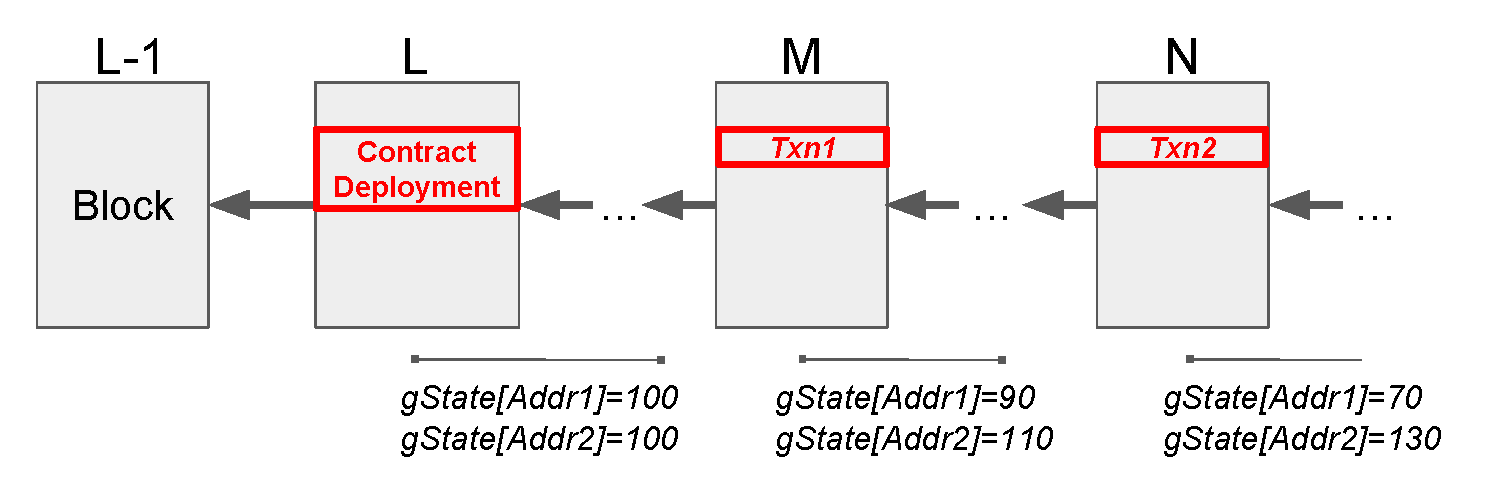
\includegraphics[width=0.9\textwidth]{diagram/provenance/contract.pdf}
  \caption{The example ledger with \textit{gState} between the block interval}
  \label{diagram:prov:ledger}
\end{figure}


\subsection{Capturing Provenance}
Blockchains support only a small set of data operators for general workloads, namely \textit{read} and \textit{write}. These operators are not provenance friendly, in the sense that they do not capture any data
association (input-output dependency). In contrast, relational databases or big data systems have many
provenance-friendly operators, such as \textit{map}, \textit{reduce} and \textit{join}, whose semantics meaningfully
capture the association. For instance, the output of \textit{join} is clearly derived from (or is dependent on)
the input data.  

\begin{figure}
    \footnotesize
    \centering
    \begin{verbatim}
    contract Token {
        method Transfer(...){...} // as above
        method prov_helper(name, reads, writes) {
          if name == "Transfer" {
            for (id,value) in writes {
                if (reads[id] < value) {
                    recipient = id;
                } else {sender = id; }
            }
            // dependency list with a 
            // single element. 
            dep = [sender];  
            return {recipient:dep};
          } 
          ...
        }
    }
    \end{verbatim}
    \caption{The provenance helper method for \textit{Token} contract}
    \subcaption*{It defines dependency between the
    sender identifier and recipient identifier. This method is invoke after every invocation of the Token
    contract.} 
    \label{code:prov:helper_contract}
\end{figure}


In {\fs}, every contract method can be made provenance-friendly via a {\em helper} method.  
More specifically, during transaction execution, {\fs} collects the identifiers and values of the
accessed states, i.e., ones used in \texttt{read} and \texttt{write} operations. The results are a read set \texttt{ 
reads} and write set \texttt{writes}. For {\em Txn1}, ${\texttt{reads}} = \{{\textit Addr1}: 100, {\textit Addr2}:
100\}$, and ${\texttt{writes}} = \{{\textit Addr1}: 90, {\textit Addr2}: 110\}$. After the execution finishes,
these sets are passed to a user-defined method \texttt{prov\_helper}, together with the name of the contract
method. \texttt{prov\_helper} has the following signature:
\begin{verbatim}
method prov_helper(name: string,
                   reads: map(string, byte[]), 
                   writes: map(string, byte[])) 
       returns map(string, string[]);
\end{verbatim}

It returns a set of dependencies based on the input read and write sets. Figure~\ref{code:prov:helper_contract}
shows implementation of the helper method for the Token contract. It first computes the identifier of the
sender and recipient from the read and write sets. Specifically, the identifier whose value in \texttt{writes} is lower than that
in \texttt{reads} is the sender, and the opposite is true for the recipient. It then returns a dependency set of
a single element: the recipient-sender dependency. In our example, for {\em Txn1}, this method returns
$\{{\textit Addr2}: [{\textit Addr1}]\}$ 

{\fs} ensures that \texttt{prov\_helper} is invoked immediately after every successfully contract execution.
If the method is left empty, {\fs} uses all identifiers in the read set as dependency of each identifier
in the write set. Interested readers may observe that the vanilla Fabric already computes for the read/write set
during the endorsement phase. 
Orthogonal to ours, they are internally used for the concurrency control to achieve one-copy serializability. 
Instead, we allow contract developers to capture for their application-level provenance. 


\subsection{Smart Contract APIs}
Current smart contracts can only safely access the {\em latest} blockchain state. In Hyperledger, for example, the \texttt{get(k)} operation returns the last value of $k$ that is written or being batched.  In Ethereum, on the other
hand, when a smart contract reads a value of $k$ at block $b$, the system considers the snapshot of states at
block $b-1$ as the latest states. Although there may exist a block $b' > b$ on a different branch, the
smart contract always treats what returned from the storage layer as the latest state.  

The main limitation of the current APIs is that the smart contract cannot tamper-evidently read previous values of a state.
Instead, the contract has to explicit track historical versions, for example by maintaining a list of versions
for every state. This approach is costly both in terms of storage and computation. {\fs} addresses this limitation with three additional smart contract APIs. 

\begin{itemize}
    \item \texttt{Hist(stateID, [blockNum])}: returns the tuple \texttt{(val, blkStart)} where \texttt{val}
    is the value of \texttt{stateID} at the snapshot of block \texttt{blockNum}. If \texttt{blockNum} is not specified, the latest block is used. \texttt{blkStart} is the index of the block that contains a transaction setting \texttt{stateID}. 

    \item \texttt{Backward(stateID, blkNum)}: returns a list of tuples \texttt{(depStateID, depBlkNum)} where \texttt{ depStateID} is the dependency state of \texttt{stateID} at block \texttt{blkNum}. \texttt{depBlkNum} is the block number at which the value of \texttt{depStateID} is set. It also returns \texttt{txID} which is the identifier of the transaction that sets \texttt{stateID}.
    In our example, \texttt{Backward(Addr2, N)} returns \texttt{(Addr1, M)} and \texttt{txID} is equal to \texttt{Txn2}. 

    \item \texttt{Forward(stateID, blkNum)}: similar to the \texttt{Backward} API, but returns the states of
    which \texttt{stateID} is a dependency and the corresponding transaction identifier. For example, \texttt{Forward(Addr1, L)} returns \texttt{(Addr2, M, Txn1)}.
\end{itemize}

\begin{figure}[t]
\footnotesize
\centering
\begin{verbatim}
contract Token {
  ...
  method Refund(addr) {
    blk := last block in the ledger
    first_blk := first block in this month
    sum = count = 0;
    while (first_blk < blk) {
      val, startBlk = Hist(addr, blk);
      blk = startBlk - 1; 
      sum += val;
      count += 1;
    }
    avg = sum / count;
    refund_amount := refund amount based on avg
    gState[addr] += refund_amount;
  }

  method Suspect(addr) {
    blk := last block in the ledger
    suspected = false;
    iterate 5 times {
      val, startBlk = Hist(addr, blk);
      for (depAddr, depBlk) 
            in (Backward(addr, startBlk) 
            or Forward(addr, startBlk)) {
        if depAddr in gState["suspect"] {
          gState["suspect"].append(addr);
          return;
        }
      }
      blk = startBlk - 1; 
    }
  }
}

\end{verbatim}
\caption{The modified \textit{Token} contract with provenance-dependent methods.}
\label{code:prov:enhanced_contract}
\end{figure}

% \subsection{Sample Usage}
Figure~\ref{code:prov:enhanced_contract} demonstrates how the above APIs are used to express smart contract logics
that are currently impossible in the secure manner.
We add two additional methods to the original contract, both of which use the new
APIs. The \textit{Refund} method examines an account's average balance in the recent month and makes the
refund accordingly. The \textit{Suspect} method marks an address as suspected if one of its last 5
transactions is with a suspected address. 



\section{Secure Provenance Storage} 
\label{sec:provenance:storage}
In this section, we discuss how {\fs} enhances existing blockchain storage layer to provide efficient
tracking and tamper evidence for the captured provenance. Our key insight is to reorganize the flat leaf
nodes in the original Merkle tree into a Merkle DAG. We first describe the Merkle DAG structure, then discuss
its properties. Finally, we explain how to exploit the blockchain execution model to support forward
provenance tracking. 

\subsection{Merkle DAG}

Let $k$ be the unique identifier of a blockchain state, whose evolution history is expected to be tracked. 
Let $v$ be the unique version number that identifies the state in its evolution history. 
When the state at version $v$ is updated, the new version $v'$ is strictly greater than $v$. 
In {\fs}, we directly use the block number as its version $v$. 
Let $s_{k,v}$ denote the value of the state with identifier
$k$ at version $v$. We drop the subscripts if the meaning of $k$ and $v$ are not important. For any $k \neq
k'$ and $v \neq v'$, $s_{k,v}$ and $s_{k',v'}$ represent the values of two different states at different versions.  
$s^b_k$ represents the state value with identifier $k$ at its latest version before block b. 
In our example, for $k=Addr1$ and $v=M$, $s_{k,v}=90$.

\begin{definition}
A transaction, identified by ${tid}$ which is strictly increasing, reads a set of input states $S^{i}_{tid}$ 
and updates a set of output states $S^{o}_{tid}$. 
A valid transaction satisfies the following properties: 
  \begin{equation}
    \label{eq:1} \forall s_{k_1,v_1}, s_{k_2,v_2} \in S^{o}_{tid}. \quad k_1 \ne k_2
    \land v_1 = v_2 
  \end{equation}
  \begin{equation}\label{eq:2}
    \forall s_{k_1,v_1} \in S^{i}_{tid}, s_{k_2,v_2} \in S^{o}_{tid}. \quad v_1 < v_2 
  \end{equation}
  \begin{equation}\label{eq:22}
    \forall s_{k,v} \in S^{i}_{tid},  s_{k,v'} \in S^{i}_{tid'}. \quad tid < tid' \Rightarrow v \le v'. 
  \end{equation}
  \begin{equation}\label{eq:3}
    tid \ne tid' \Rightarrow S^{o}_{tid} \cap S^{o}_{tid'} = \emptyset
  \end{equation}
\end{definition}

Property (\ref{eq:1}) means that the versions of all output states of a transaction are identical, 
because they are updated by the same transaction in the same block. 
Property (\ref{eq:2}) implies the version of any input state is strictly lower than
that of the output version. This makes sense because the blockchain establishes a total order over the
transactions, and because the input states can only be updated in previous transactions. 
Property (\ref{eq:22}) specifies that, for all the states with the same identifier, the input of later
transactions can never have an earlier version.  This ensures the input state of any transaction must be
up-to-date during execution time.  Finally, Property (\ref{eq:3}) means that every state update is  unique. 

\begin{definition}
The dependency of state $s$ is a subset of the input states of the transaction that outputs $s$. More
specifically: 
  \begin{displaymath}
    dep(s) \subset S^{i}_{tid} \ \text{where} \ s \in S^{o}_{tid}. 
  \end{displaymath}
\end{definition}
\noindent We note that $dep$, which is returned by \texttt{prov\_helper} method, is only a subset of the read
set.  

\begin{definition} \label{def:entry}
The entry $E_{s_{k,v}}$ of the state $s_{k,v}$ is a tuple containing the current version, the state value, and the
hashes of the entries of its dependent state. More specifically:
  \begin{displaymath}
    E_{s_{k,v}}= \langle v, s_{k,v}, \{hash(E_{s'})|s' \in dep(s_{k,v})\} \rangle
  \end{displaymath}
\end{definition}
\noindent An entry uniquely identifies a state. In {\fs}, we associate each entry with its corresponding
hash. 

\begin{definition}
The set of latest states at block $b$, denoted as $S_{latest,b}$ is defined as: 
  \begin{displaymath}
    S_{latest, b} = \bigcup\limits_{k}\{s^b_k\}
    % S_{latest, b} = \Union \{s^*_k\}
  \end{displaymath}
\end{definition}
\noindent Let $U_b$ be the updated states in block $b$. We can compute $S_{latest, b}$ by recursively
combining $U_b$ with $S_{latest, b-1} \setminus U_b$.  

\begin{definition}
$\chi_b$ is the root of a Merkle tree built on the map $S_b$ where 
  \begin{displaymath}
  S_b = \{k:hash(E_{s^b_{k}}) | \forall s^b_{k} \in S_{latest, b}\}. 
  \end{displaymath}
\end{definition}

{\fs} stores $\chi_b$ as the state digest in the block header. Figure~\ref{diagram:prov:dag} illustrates how state DAG evolves with the blockchain.

\begin{figure}
  \centering
  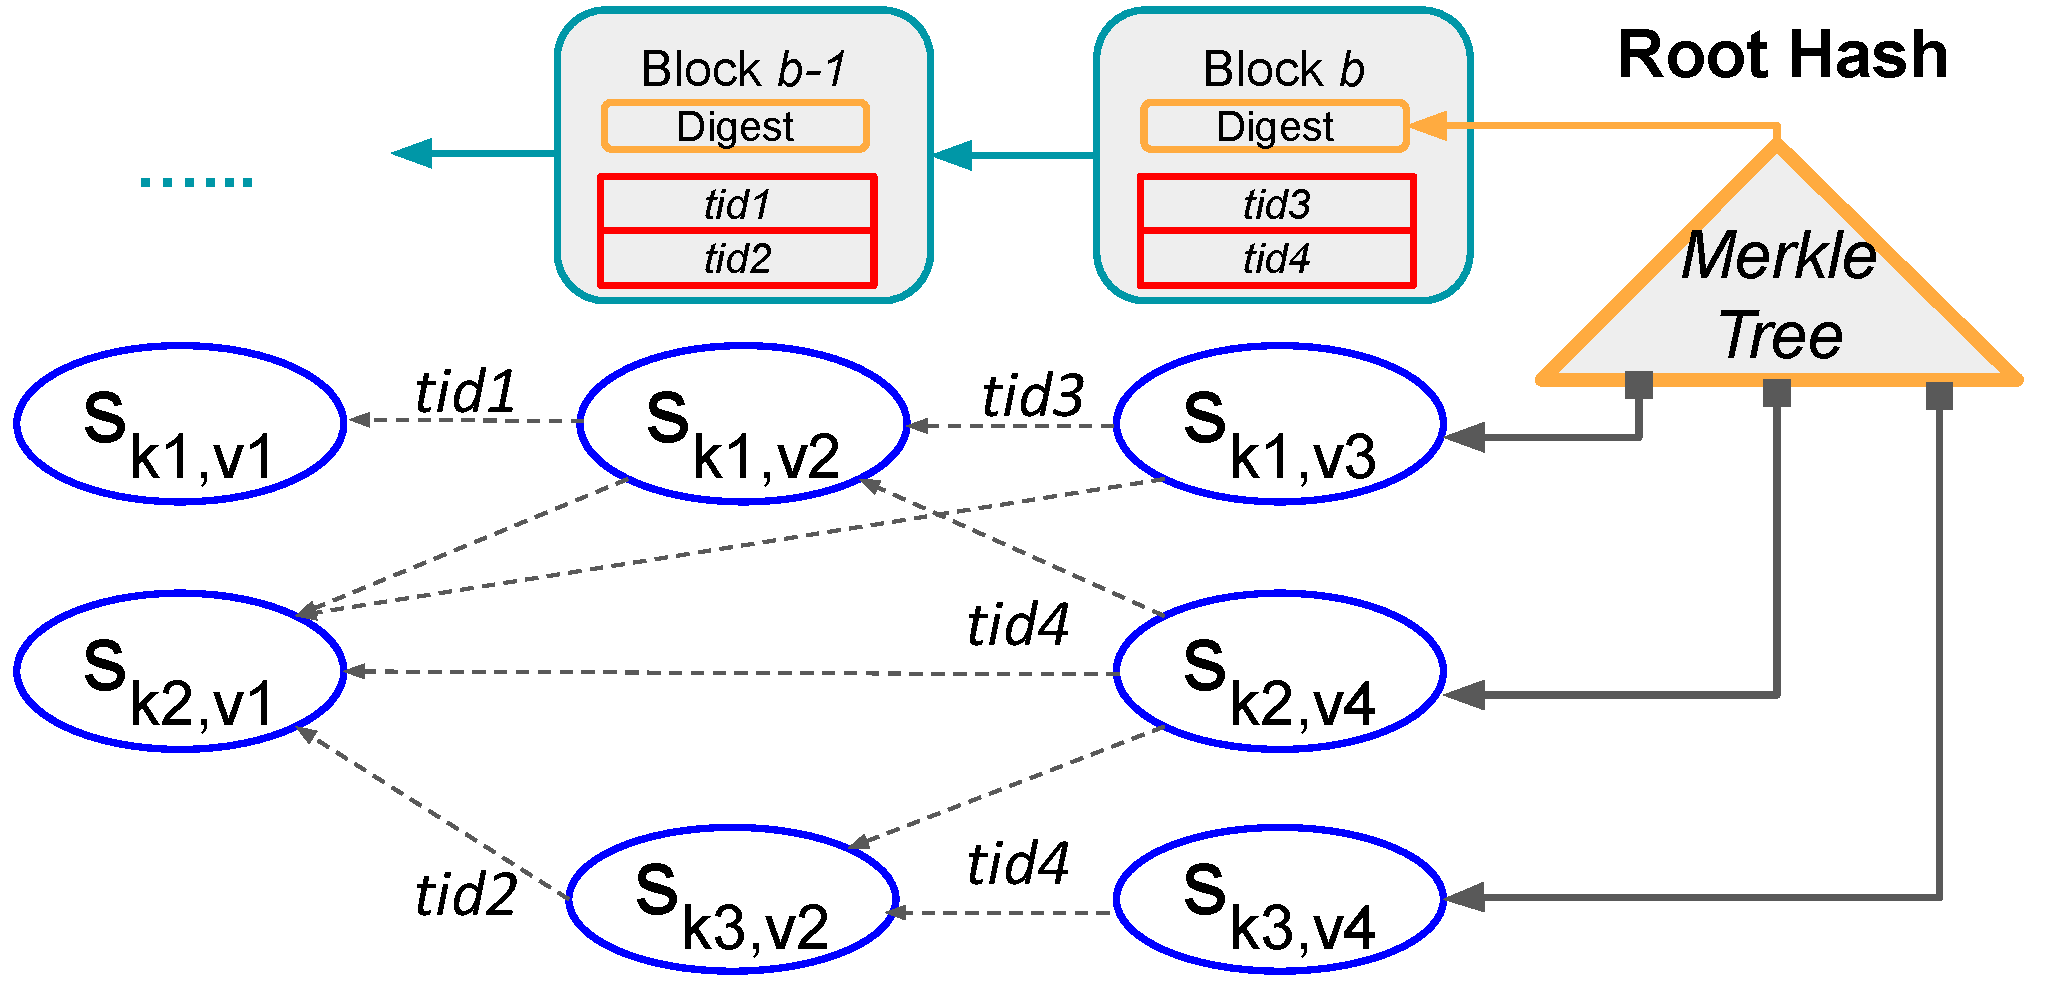
\includegraphics[width=0.9\textwidth]{diagram/provenance/DAG.pdf}
\caption{A Merkle DAG for storing provenance. }
\subcaption*{$s_{k_2,v_4}$ and $s_{k_3,v_4}$ updated by the same transaction ($tid_4$), but their dependencies are
different. $b$ contains two transactions, $tid_3$ and $tid_4$. Its latest states include $s_{k_1,
v_3}$, $s_{k_2,v_4}$, $s_{k_3,v_4}$, from which a Merkle tree is built.} 
\label{diagram:prov:dag} 
\end{figure}

\subsection{Discussion}
Our new Merkle DAG can be easily integrated to existing blockchain index structures. In particular, existing
Merkle index such as MPT stores state values directly at the leaves, whereas the Merkle DAG in {\fs} stores
the entry hashes of the latest state versions at the leaves. By adding one more level of indirection, we
maintain the three properties of the index (tamper evidence, incremental update and snapshot), while enhancing
it with the ability to traverse the DAG to extract fine-grained provenance information. 

Recall that the state entry hash captures the entire evolution history of the state. Since this hash is
protected by the Merkle index for tamper evidence, so is the state history.  In other words, we add integrity
protection for provenance without any extra cost to the index structure.  For example, suppose a
client wants to read a specific version of a state, it first reads the state entry hash at the latest block.
This read operation can be verified against tampering, as in existing blockchains. Next, the client traverses
the DAG from this hash to read the required version. Because the DAG is tamper evident, the integrity of the
read version is guaranteed.

\subsection{Support for Forward Tracking}
\label{sec:provenance:storage:forward}
One problem of the above DAG model is that it does not support forward tracking, because the hash pointers
only reference {\em backward} dependencies. When a state is updated, these backward
dependencies are permanently established, so that they belong to the immutable derivation history of the
state. However, the state can be read by future transaction, therefore its forward dependencies cannot be
determined at the time of update. 

\begin{figure}
  \centering
  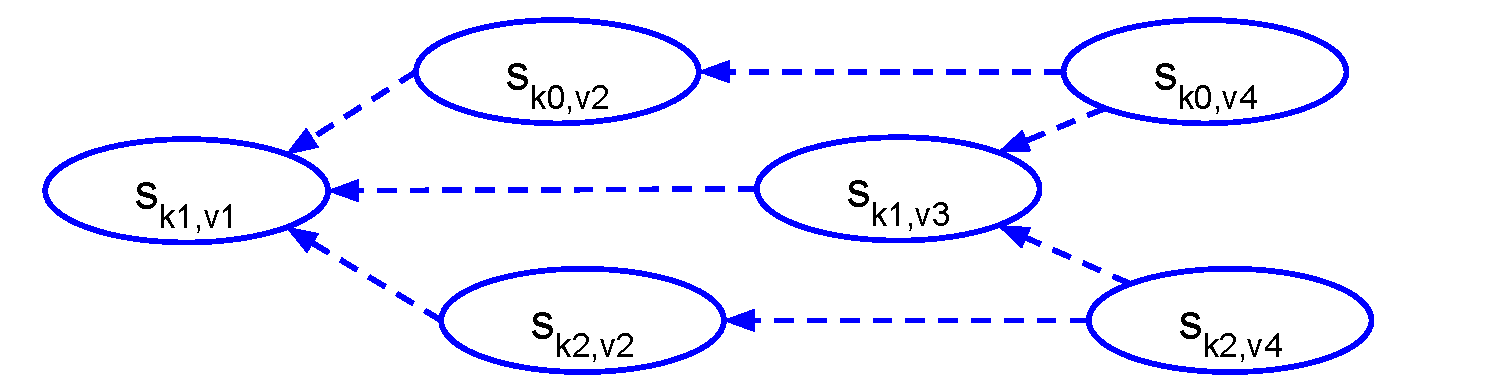
\includegraphics[width=0.9\textwidth]{diagram/provenance/forward.pdf}
  \caption{Forward tracking support for data provenance}
  \label{diagram:prov:forward}
  \subcaption*{After $s_{k_1,v_1}$ is updated, there can only be $s_{k_0,v_2}$ and
  $s_{k_2,v_2}$ that are dependent on $s_{k_1,v_1}$. Future states can only depend on $s_{k_1,v3}$. Forward
  pointers of $s_{k_1,v_1}$ are stored in the entry of $s_{k_1,v_3}$. } 
\end{figure}

Our key insight here is that only forward dependencies of the {\em latest state} are mutable. Once the state
is updated, due to the execution model of blockchain smart contract, in which the latest state is always read,
forward dependencies of the previous state version becomes permanent. As a result, they can be included into
the derivation history. Figure~\ref{diagram:prov:forward} illustrates an example, in which forward dependencies of
$s_{k_1, v_1}$ becomes fixed when the state is updated to $s_{k_1, v_3}$. This is because when the transaction
that
outputs $s_{k_0, v_4}$ is executed, it reads $s_{k_1, v_3}$ instead of $s_{k_1, v_1}$. 

In {\fs}, for each state $s_{k,v}$ at its latest version, we buffer a list of forward pointers to the
entries whose dependencies include $s_{k,v}$.  We refer to this list as $F_{s_{k,v}}$, which is defined more precisely as
follows: 
\begin{displaymath}
F_{s_{k,v}} = \{hash (E_{s'}) | s_{k,v} \in dep(s')\}
\end{displaymath}
\noindent When the state is updated to $s_{k,v'}$ for $v' > v$, we store $F_{s_{k,v}}$ at the entry of
$s_{k,v'}$.  

\section{Efficient Provenance Queries}
\label{sec:provenance:index}
The Merkle DAG structure supports efficient access to the latest state version, since the state index at block
$b$ contains pointers to all the latest versions at this block. To read the latest version of $s$, one simply
reads $\chi_b$, follows the index to the entry for $s$, and then reads the state value from the entry.
However, querying an arbitrary version in the DAG is inefficient, because one has to start at the DAG head
and traverse along the edges towards the requested version.  Supporting fast version queries is important
when the user wants to examine the state history only from a specific version (for auditing purposes, for
example).  It is also important for provenance-dependent smart contracts because such queries directly affect
contract execution time. 

In this section, we describe a novel index that facilitates fast version queries. The index is designed for
permissioned blockchains. We discuss its efficiency and how to extend it to permissionless blockchains. 

\subsection{Deterministic Append-Only Skip List} 
We propose to build an index on top of a state DAG to enable fast version queries. The index has a skip list
structure, which we call Deterministic Append-only Skip List (or DASL). It is designed for blockchains,
exploiting the fact that the blockchain is append-only, and randomness is not well
supported~\cite{cachin2016non}. More specifically, a DASL has two distinct properties compared to a normal skip
list. First, it is append-only. The index keys of the appended items, which are versions in our case, are
strictly increasing. Second, it is deterministic, that is,
the index structure is uniquely determined by the values of the appended items, unlike a stochastic skip list.
For ease of explanation, we assume that version numbers are positive integers.

\begin{definition}\label{def:1}
  Let $V_k = \langle v_0, v_1, ...\rangle$ be the sequence of version numbers of states with identifier $k$, in which $v_i <
  v_j$ for all $i<j$. A DASL index for $k$ consists of $N$ linked lists $L_0, L_1,.., L_{N-1}$. Let $v^{i}_{j-1}$ and $v^i_j$ be
  the versions in the $(j-1)^{\textit{th}}$ and $j^{\textit{th}}$ node of list $L_i$. Let $b$ be the base number, a system-wide parameter. The content
  of $L_i$ is constructed as follows:
 
  1) $v_0 \in L_i$

  2) Given $v^i_{j-1}$, $v^i_j$ is the smallest version in $V_k$ such that: 
  \begin{equation}\label{eq:4}
    \floor*{\frac{v^i_{j-1}}{b^i}} < \floor*{\frac{v^i_j}{b^i}}
  \end{equation}
\end{definition}

\begin{figure}
  \centering
  \footnotesize
  \begin{verbatim}
  struct Node {
    Version v;
    Value val;
    List<Version> pre_versions;
    List<Node*> pre_nodes;
  }
  \end{verbatim}
  \caption{Node structure that captures a state $s_{k,v}$ with value $val$}
  \label{code:prov:node}
\end{figure} 

\begin{figure}
  \centering
  \begin{subfigure}{0.32\textwidth}
    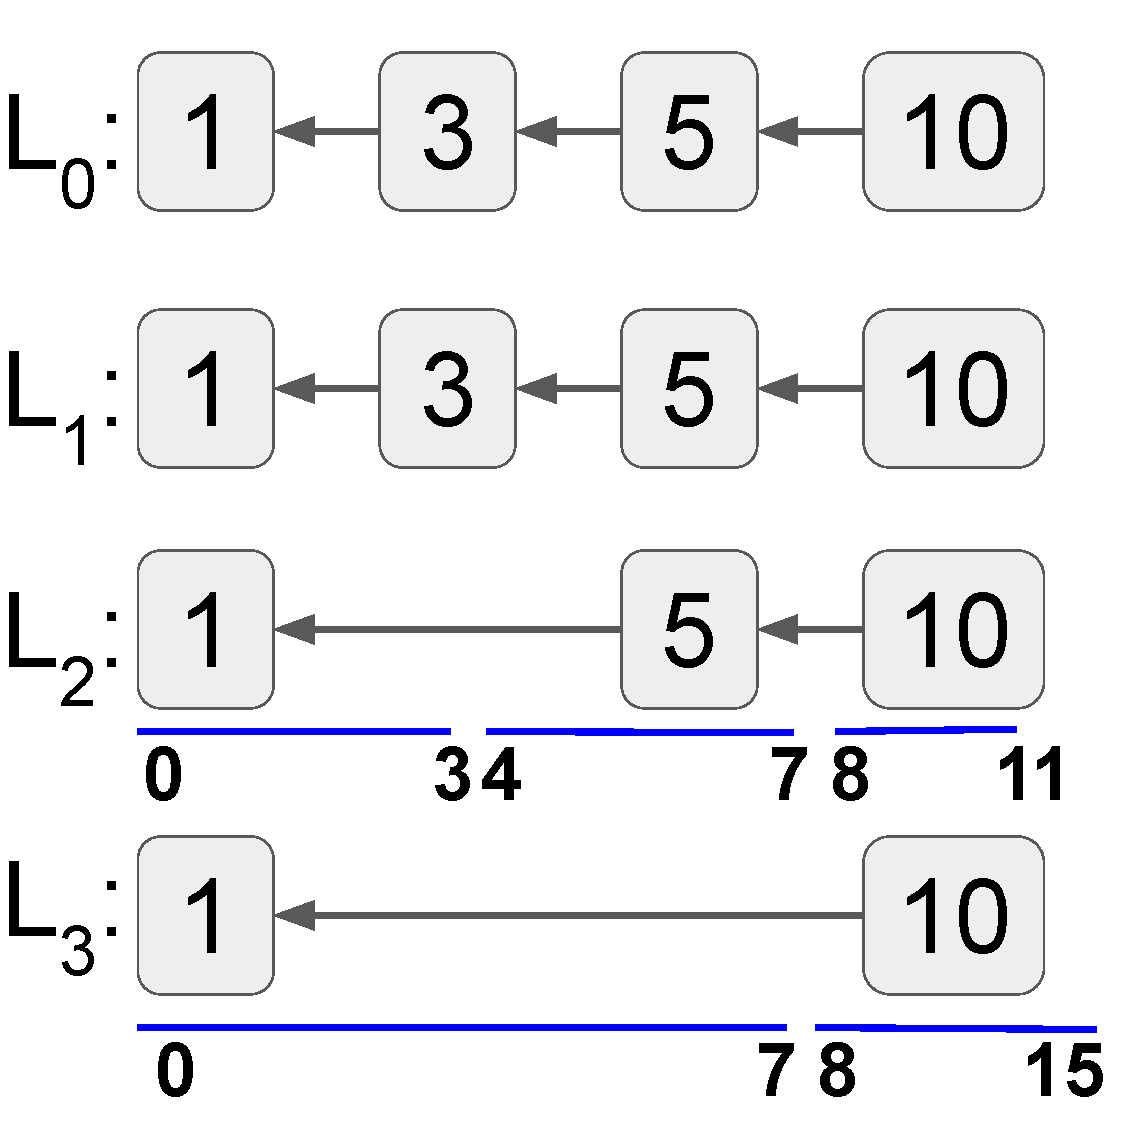
\includegraphics[width=0.99\textwidth]{diagram/provenance/dasl_original.pdf}
    \caption{}
    \label{diagram:prov:dasl_original}
  \end{subfigure}
  \begin{subfigure}{0.54\textwidth}
    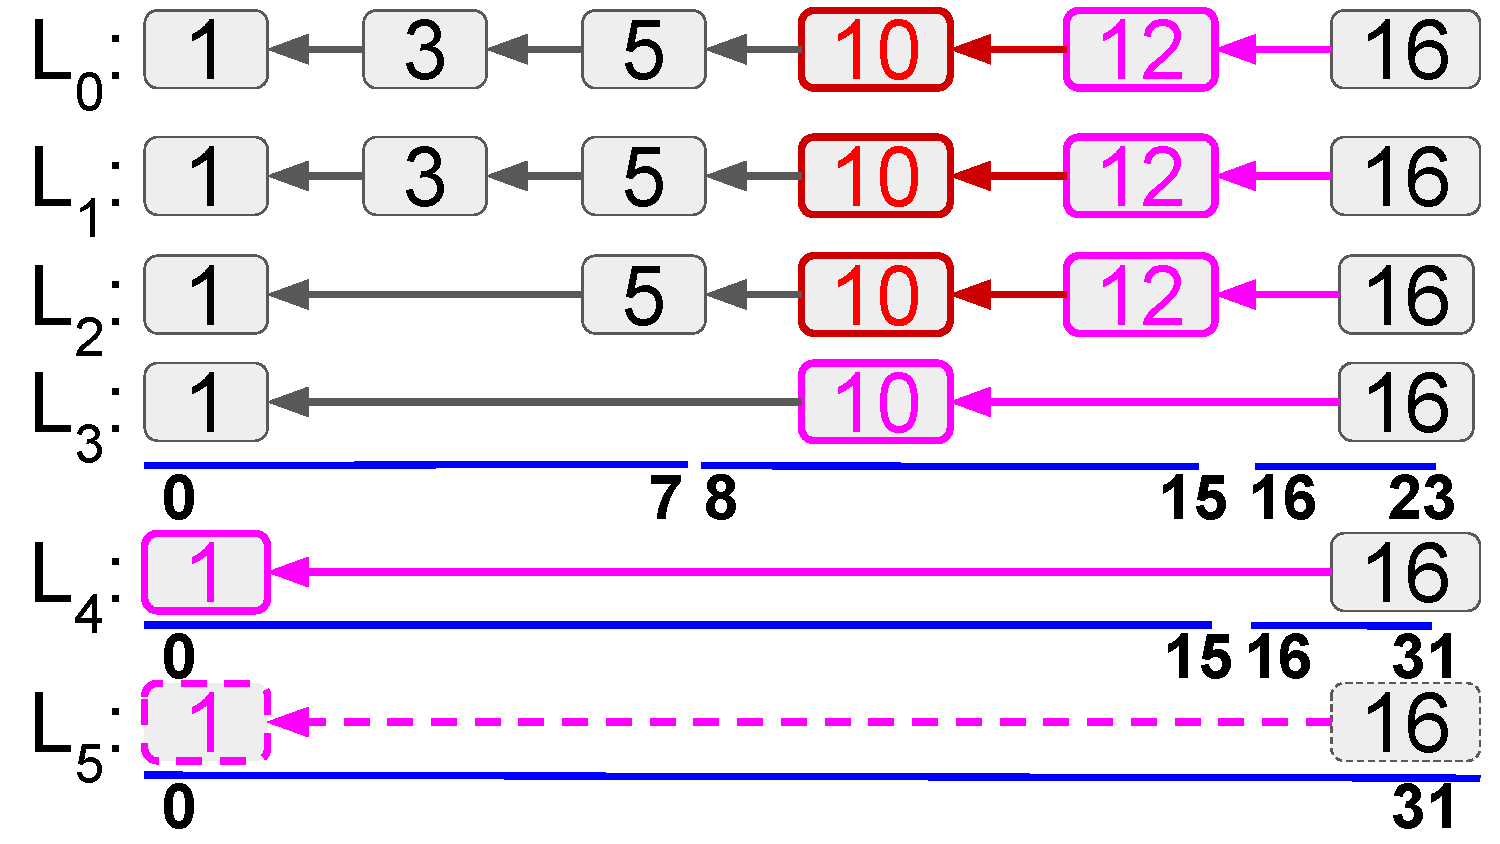
\includegraphics[width=0.99\textwidth]{diagram/provenance/dasl_appended.pdf}
    \caption{}
    \label{diagram:prov:dasl_appended}
  \end{subfigure}
  \caption{An example of the append procedure in Deterministic Append-only Skip List (DASL)}
  \subcaption*{(a) A DASL containing versions 1, 3, 5 and 10. The base $b$ is 2. The intervals for $L_2$ and
  $L_3$ are shown in blue lines. (b) The new DASL after appending version 12 and 16. $L_4$ is created when appending version $16$. $L_5$ is created, then discarded.} 
\end{figure}

Figure~\ref{code:prov:node} shows how DASL is stored with the state in a data structure called Node.  This structure
(also referred to as node) consists of the state version and value. A node belongs to multiple lists (or
levels), hence it maintains  a list of pointers to some version numbers, and another list of pointers to other
nodes.  Both lists are of size $N$, and the $i^{\textit th}$ entry of a list points to the previous version
(or the previous node) of this node in level $L_i$.  For the same key, the version number uniquely identifies
the node, hence we use version numbers to refer to the corresponding nodes.

We can view a list as consisting of continuous, non-overlapping intervals of certain sizes. In particular, the
$j^{\textit{th}}$ interval of $L_i$ represents the range $R^i_j = [jb^i, (j+1)b^i)$. Only the smallest version in $V_k$ that
falls in this range is included in the list. Figure~\ref{diagram:prov:dasl_original} gives an example of a DASL
structure with $b=2$. It can be seen that when the version numbers are sparsely distributed, the lists at lower levels are
identical. In this case, $b$ can be increased to create larger intervals which can reduce the overlapping among
lower-level lists.   

A DASL and a skip list share two properties. First, if a version number appears in $L_i$, it also appears in
$L_j$ where $j<i$.  Second, with $b=2$, suppose the last level that a version appears in is $i$, then this
version's preceding neighbour in $L_i$ appears in $L_j$ where $j>i$. 
Given these properties,
a query for a version in the DASL is executed in the same way as in the skip list.
More specifically, the query traverses a high-level list as much as possible, starting from
the last version in the last list. It moves to a lower level only if the preceding version in the current list
is strictly smaller than the requested version. In DASL, the query for version $v_q$ returns the largest
version $v \in V_k$ such that $v \leq v_q$ (the inequality occurs when $v_q$ does not exist). This result
represents the value of the state which is visible at time of $v_q$. 

\begin{algorithm}[t]
  \caption{DASL Append}
  \label{alg:prov:append}
  %uint b \tcp{base}
  \KwIn{version $v$ and last node $last$}
  \KwOut{previous versions and nodes}
  $\textit{level}$=0;\   \tcp{list level} 
  $\textit{pre\_versions}$ = []\;
  $\textit{pre\_nodes}$ = []\;
  $\textit{finish}$ = false \;
  $\textit{cur} = \textit{last}$ \;
  \While{not finish} {
    $l$ = $\textit{cur}$->$\textit{pre\_versions.size()}$ \;
    \If {l > 0} {
      \For {j=level; j<l; ++j} { \label{alg:prov:append:iterate_begin}
        \If {$\textit{cur}$->$\textit{version}$ / $b^j$ < $v$ / $b^j$} {
          $\textit{pre\_versions}$.append($\textit{cur}$->$\textit{version}$)\;
          $\textit{pre\_nodes}$.append($\textit{cur}$)\;
        } \Else {
          $\textit{finish}$ = true\;
          break\;
        }
      }
      \If {not finish} {
        $\textit{cur}$ = $\textit{cur}$->\textit{pre\_versions[l-1]}\;
        $\textit{level}=l$
      } \label{alg:prov:append:iterate_end}
    } \Else {
      \tcc {We have reached the last level}
      $\textit{finish}$ = true\;
      \While {$\textit{cur}$->$\textit{version}$ / $b^{\textit{level}}$ < $v$ / $b^{\textit{level}}$} { \label{alg:prov:append:head_begin}
        ++$\textit{level}$\;
        $\textit{pre\_versions}$.append($\textit{cur}$->$\textit{version}$)\;
        $\textit{pre\_nodes}$.append($\textit{cur}$)\;
      }\label{alg:prov:append:head_end}
    }
  }

  \Return{$pre\_version$, $pre\_nodes$;}
\end{algorithm}

We now describe how a new node is appended to DASL. The challenge is to determine the lists that should include the
new node. Algorithm \ref{alg:prov:append} details the steps that find the lists, and subsequently the previous
versions, of the new node. The key idea is to start from the last node in $L_0$, then keep increasing the list
level until the current node and the new node belong to the same interval (line
\ref{alg:prov:append:iterate_begin} - \ref{alg:prov:append:iterate_end}). Figure~\ref{diagram:prov:dasl_appended} shows the result of appending a node with version $12$ to the original DASL. The algorithm starts at node $10$ and moves up to list $L_1$ and $L_2$. It stops at $L_3$ because in this level node $10$ and $12$ belong to the same
interval, i.e., $[8,16)$. Thus, the new node is appended to list $L_0$ to $L_2$. When the algorithm reaches
the last level and is still able to append, it creates a new level where node $0$ is the first entry and
repeats the process (line \ref{alg:prov:append:head_begin} -
\ref{alg:prov:append:head_end}). In Figure~\ref{diagram:prov:dasl_appended}, when appending version $16$, all existing lists can be used. The algorithm then creates $L_4$ with node $1$ and appends the node $16$ to it. It also creates
level $L_5$, but then discards it because node $16$ will not be appended since it belongs to same
interval of $[0,32)$ with node $1$. 

\subsection{Discussion} \label{sec:provenance:model_discuss}
\textbf{Integrating to Merkle DAG. } 
The DASL is integrated to the Merkle DAG as follows. The node structure (Figure \ref{code:prov:node}) is stored in
the state entry (Definition~\ref{def:entry}).  The node pointers are implemented entry hashes. The Merkle tree
structure remains unchanged.  

\textbf{Speed-storage tradeoff. } 
As a skip list variant, DASL shares the same lineage space complexity and 
logarithmic query time complexity. 
Suppose there are $v^*$ number of versions and the base of DASL is $b$. 
The maximum number of required pointers is $\frac{bv^*-1}{b-1}$. 
(There are at most $\ceil{\log_b v^*}$ levels and the $i$-th level takes at most $\ceil{\frac{v^*}{b^i}}-1$ pointers.)
Suppose the queried version is $v^q$ and the query distance $d=v^*-v^q$, the maximum number of hops in such query is capped at $2b\ceil{\log_b d}$. (A query traversal from the end will undergo two stages, one stage towards lower levels  and the other stage back towards upper levels. In each stage, 
the traversal will take at most $b$ hops on the same list before moving to the next level.
And there are at most $\ceil{\log_b d}$ levels to traverse.)
Hence, $b$ controls the tradeoff between the space overhead and query delay. 
One benefit of this property is that DASL queries favor more recent
versions, i.e. $d$ are small.
It is useful for smart contracts that work on recent rather than old versions.  
Another benefit is that the performance of such recent-version queries does not change as the state history grows.  

\textbf{Extending to permissionless blockchains. } 
We note that DASL incurs storage overhead. The version query also incurs some computation cost, even though it
is more efficient with DASL than without it. These costs may be small enough such that they do not
affect the performance of a permissioned blockchain, as we demonstrate in Chapter~\ref{sec:provenance:exp}.  However,
they need to be carefully managed in a permissionless blockchain where any overhead directly translates to
monetary cost to the miners. In particular, any additional cost to the miner triggers the Verifier
Dilemma~\cite{luu2015demystifying} and compromises the incentive mechanism of the blockchain.  

A malicious user could issue a transaction that references a very old version. Reading earlier versions is more
expensive, because there are more hops involved. This overhead is born by all nodes in the network,
since every node in the network has to execute the same transaction. Current public blockchains prevent such
denial-of-service attack by explicitly charging a fee for each operation in the transaction. In Ethereum, the
transaction owner pays for the resource consumption in {\em gas}. A transaction that writes more data or
consumes more CPUs has to pay more {\em gas}. Thus, rational users are deterred from running too complex
transactions on the blockchain. 

As DASL consumes resources, its costs must be explicitly accounted for in permissionless blockchains.
More specifically, during deployment, the contract owner specifies which states require DASL support.
Alternatively, DASL support can be automatically inferred from the contract's source code. The deployment fee
should reflect this extra storage cost for DASL. If the fee is too high, the owner can lower it by increasing
b. During contract execution, the execution engine must charge the cost of DASL queries to the transaction
fee. In particular, a query that requires more hops to find the requested version incurs a higher transaction
fee. Users may empirically estimate the hops (as well as the cost) based on the above-derived theoretical upper bound. 

\section{Implementation}
\label{sec:provenance:implementation}
\begin{figure}
  \centering
  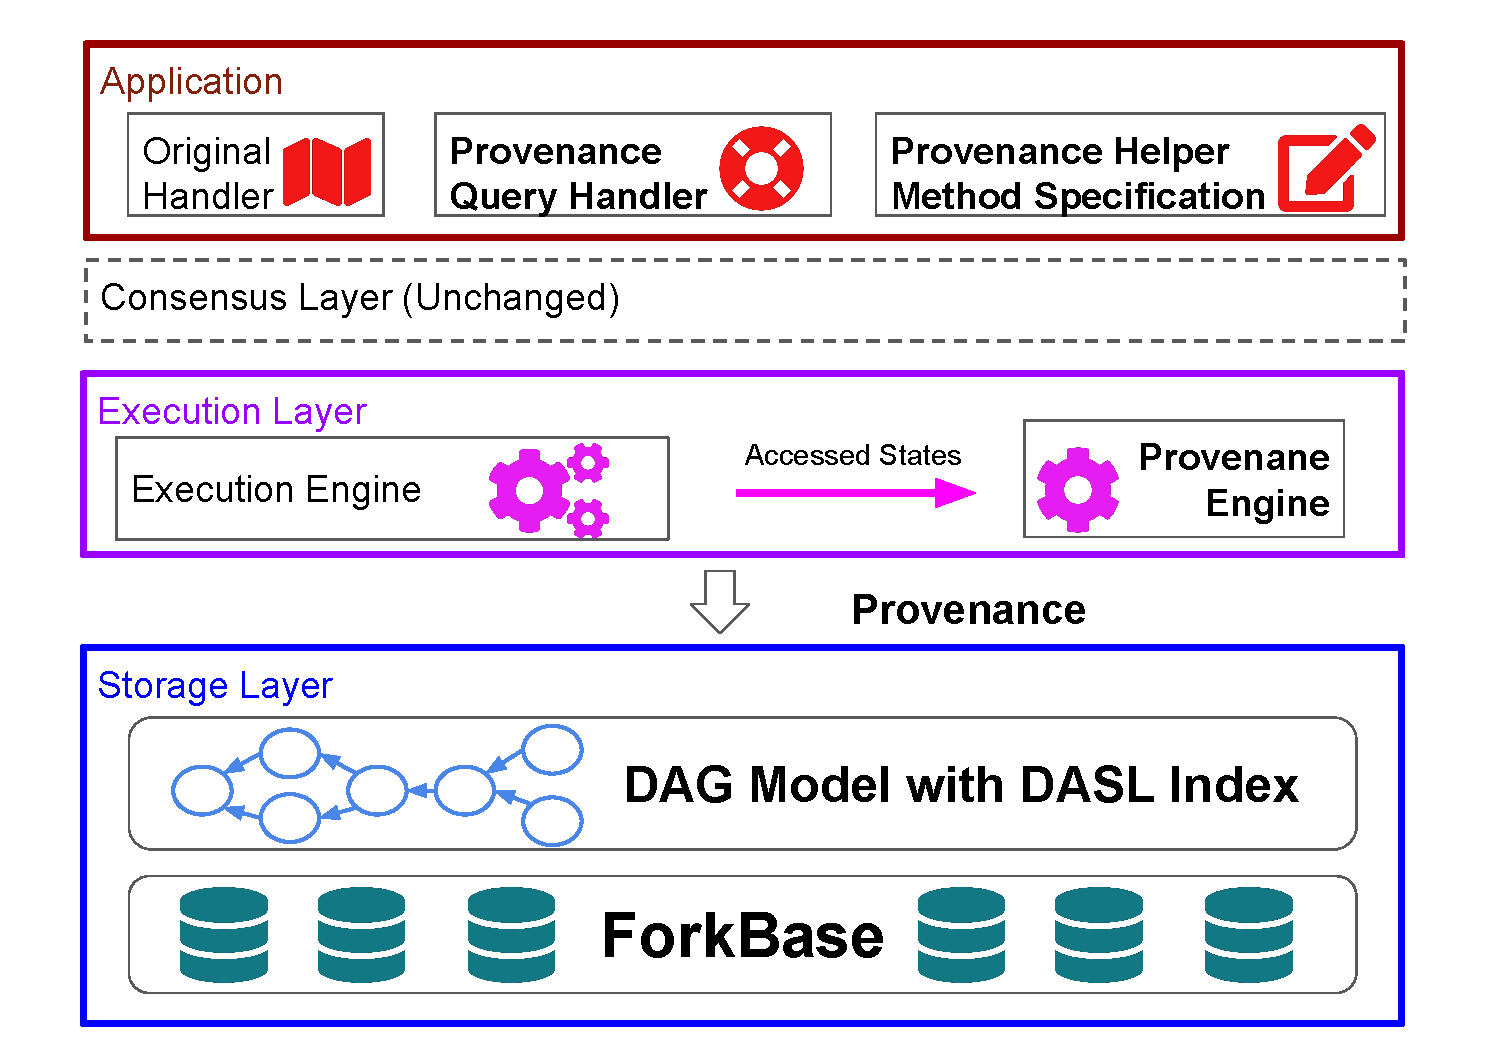
\includegraphics[width=0.8\textwidth]{diagram/provenance/lineagechain.pdf}
  \caption{The {\fs}'s instrumentation on Fabric to support data provenance }
  \subcaption*{The original storage layer is replaced with the implementation that
  supports fine-grained provenance. The original execution layer is instrumented with a provenance capture
  engine. The application layer contains the new helper method and provenance query APIs. The consensus layer is unchanged. } 
  \label{diagram:prov:arch} 
\end{figure}

\begin{algorithm}
  \caption{Provenance update and digest Computation} \label{prov:fabric_change} 
  \tcc{fb is the shorthand for ForkBase. fb.Map is the built-in map data type in Forkbase.}     
  fb.Map<id,vid> $\textit{latest}$\;
    String $\textit{branch}$ = "default"\;
    \tcp{Buffered forward pointers}
    Map<id, List<vid>> $\textit{forward}$\;  
  
    \KwIn{$\textit{id}$, $\textit{version}$, $\textit{value}$ of the updated state}
    \KwIn{ids of the dependent states, $\textit{dep\_ids}$}
    \SetKwFunction{FUpdate}{Update}
    \SetKwProg{Fn}{Function}{:}{}
    \Fn{\FUpdate{id, version, value, dep\_ids}}{
     \tcc {Backward pointers}
      List<vid> $\textit{back\_vids}$\; \label{lst:line:back_begin}
      \For {$\textit{dep\_id}$ in $\textit{dep\_ids}$} {
        $\textit{back\_vid}$ = $latest$[$\textit{dep\_id}$]\;
        $\textit{back\_vids}$.push\_back($\textit{back\_vid}$)\;
      } \label{lst:line:back_end}
      \tcc{Forward pointers}
      $\textit{forward\_vids}$ = $\textit{forward[id]}$\; \label{lst:line:forward}
      \texttt{\\}
   
      \tcc{Retrieve pointer to last DASL node}
      $\textit{last\_vid}$ = $latest$[$\textit{id}$]\;  \label{lst:line:dasl_begin}
      \tcc{Refer DASL Append in Algorithm \ref{alg:prov:append}}
      $\textit{pre\_versions}$, $\textit{pre\_vids}$ = DaslAppend($\textit{version}$, $\textit{last\_vid}$)\; 
      $\textit{node}$ = new DaslNode\{$version$, $pre\_versions$, $pre\_vids$\} \;\label{lst:line:dasl_end}
      $\textit{meta}$ = Serialize($\textit{back\_vids}$, $\textit{forward\_vids}$, $node$) \;  \label{lst:line:dump_begin}
  
      \texttt{\\}
      \tcc{Store the updated value}
      $\textit{new\_vid}$ = fb.Put($\textit{id}$, $\textit{branch}$, $\textit{value}$, $\textit{meta}$)\;  \label{lst:line:dump_end}
  
      \texttt{\\}
      \tcc{Update forward pointers}
      \For {$\textit{dep\_id}$ in $\textit{dep\_ids}$} {  \label{lst:line:forward_begin}
        $\textit{forward[dep\_id]}$.push\_back($\textit{new\_vid}$);
      }
  
      $\textit{forward[id]}$.Clear()\;  \label{lst:line:forward_end}
      $\textit{latest[id]}$ = $\textit{new\_vid}$\;  \label{lst:line:latest}
    }
    \texttt{\\}
    \KwOut{The state digest for the committed block}
    \SetKwFunction{FCommit}{ComputeDigest}
    \Fn{\FCommit{}}{
      $\textit{latest\_vid}$ = fb.Put("state", $\textit{branch}$, $\textit{latest}$, nil)\;
      \Return{$\textit{latest\_vid}$}\;
    }
\end{algorithm}
In this section, we present our implementation of {\fs} based on Hyperledger Fabric v2.2. 
Figure~\ref{diagram:prov:arch} highlights our changes in a layer-wise fashion. 
In particular, we completely
replace the storage layer with our implementation of the Merkle DAG and DASL index. This new storage
is built on top of ForkBase~\cite{wang2018forkbase}, a state-of-the-art blockchain storage system
with support for version tracking.  We instrument the original execution engine to record read and write sets
during contract execution. At the application layer we add a new helper method and three provenance APIs. The
execution engine is modified to invoke the helper method after every successful contract execution.  


\subsection{Storage Layer}
Instead of implementing the storage layer from scratch, we leverage ForkBase for its support of version
tracking.  We exploit three properties of ForkBase in {\fs}. The first is the fork semantics, with which
the application can specify a \textit{branch} for the update. Given
a branch, ForkBase provides access to the latest value.  The second property is tamper evidence, in which
every update returns a tamper-evident identifier {\em vid} which captures the entire evolution history of the
updated value. A data object in ForkBase is uniquely identified by the key and {\em vid}. In {\fs}, {\em
vid} is used as the entry hash in the DAG, and as the pointer in DASL. The third property is the rich set of
built-in data types including map, list and set. 
Figure~\ref{code:prov:api} lists our utilized ForkBase APIs with their explanations. 

\begin{figure}
\centering
\footnotesize
\begin{verbatim}
// Update the value for key in a branch with the metadata 
//   and return a tamper-evident vid. 
// Value can be a primitive like a string, or more complex types like map, list, etc. 
vid <- Put(key, branch, value, metadata);
// Retrieve the latest value for a key on a branch
value <- GetLastValue(key, branch);
// Retrieve the value or the metadata for a key based on vid. 
value <- GetValue(key, vid);
meta <- GetMetadata(key, vid);
\end{verbatim}
\caption{ForkBase APIs to implement the {\fs}'s storage}
\subcaption{\textit{metadata} is a user provided string that describes the updated value. And \textit{vid} is uniquely determined by the updated value, key, branch and the metedata. }
\label{code:prov:api}
\end{figure}

Algorithm~\ref{prov:fabric_change} details our implementation for updating states
and computing the global state digest when a block is being
committed. The update function is invoked with a new state
and a list of dependencies. We first prepare the list of backward pointers by retrieving the latest {\em vids} of the dependent
states (line~\ref{lst:line:back_begin}-\ref{lst:line:back_end}). Next, we build the pointers for the DASL
index, then retrieve the forward pointers
of the previous state (line~\ref{lst:line:forward}). The metadata from these steps are serialized and stored together with the updated
value in ForkBase (line~\ref{lst:line:dump_begin}-\ref{lst:line:dump_end}). The result is a new {\em vid} for
the update, which is appended to the list of forward pointers of every dependent state
(line~\ref{lst:line:forward_begin}-\ref{lst:line:forward_end}). {\em vid} is now 
the latest version (line \ref{lst:line:latest}). 

The global states are stored in a map object in ForkBase. To compute the global state digest, we simply update
the map object with the new {\em vids} computed for this block. The update operation of the map object, which
is built as a Merkle tree in ForkBase, returns a digest {\em latest\_vid} which is then included
to the block header.  This digest provides tamper evidence for the evolution histories of all the states up to
the current block.
Given a {\em key}, the query on its latest value can be directly answered by \textit{fb.GetLastValue(key, branch="default")}. For the historical value and dependency, one must locate the corresponding {\em vid} for that entry. 
DASL facilitates this query process. 
Then one shall use {\em vid} to fetch for the value and metadata with the corresponding ForkBase APIs. 

\subsection{Application and Execution Layer}
In {\fs}, users write their smart contracts by implementing the \texttt{Chaincode} interface. Given any  \texttt{Chaincode} implementations, the execution engine triggers the \texttt{Init} and \texttt{Invoke} method during deployment and
invocation respectively. Both methods take as input an instance of \texttt{ChaincodeStubInterface} which
supplies relevant context, such as access to the ledger states, to the smart contract. 

We add the helper method, called \texttt{ProvHelper}, to the \texttt{Chaincode} interface. This method's signature,
and how to write user-defined provenance rules with it, are explained in Chapter~\ref{sec:provenance:capture}. The
execution engine intercepts \texttt{PutState} and \texttt{GetStates} during execution to record the read set and the
write set. It invokes \texttt{ProvHelper} when the execution finishes. Then it piggybacks the computed dependency along with the transaction, later to be stored securely when the transaction commits. Fig
The three new provenance APIs, namely \texttt{Hist}, \texttt{Backward} and \texttt{Forward}, are added to \texttt{ChaincodeStubInterface}
and therefore previously-stored provenance is accessible to all contract methods. 
Appendix~\ref{sec:append:contracts:stub} and~\ref{sec:append:contracts:token} attaches the code of the provenance APIs introduced in \texttt{ChaincodeStubInterface}, and the full-fledged chaincode for the \textit{Token} contract in Figure~\ref{code:prov:enhanced_contract}

\section{Performance Evaluation}
\label{sec:provenance:exp}
\subsection{Baselines and Experimental Setup}
\label{sec:provenance:exp:setup}

We evaluate {\fs} against two baselines. 
The first baseline is the original Fabric, without any provenance support.
The second one, which we refer as {\fsPr}, directly enhances the original storage engine LevelDB for the provenance. 
To be specific, previously Fabric associates the state IDs only with their latest values in LevelDB. 
With our modification, historical values and dependencies are now associated with the concatenations of their IDs and versions. 
For example, with respect to the example in Figure~\ref{diagram:prov:dag}, the storage entries (in the format of \textit{key:value}) for state ID $k_1$ are organized as follows: 
\begin{equation*}
  \begin{aligned}
    Hist\_k1\_v1: S_{k1\_v1} \\
    Hist\_k1\_v2: S_{k1\_v2} \\
    Hist\_k1\_v3: S_{k1\_v3} \\
    Backward\_k1\_v1: \{\} \\
    Backward\_k1\_v2: \{k1\_v1,k2\_v1\} \\
    Backward\_k1\_v3: \{k1\_v2,k2\_v1\} \\
    Forward\_k1\_v1: \{k1\_v2\} \\
    Forward\_k1\_v2: \{k1\_v3, k2\_v4\} \\
    Forward\_k1\_v3: \{\} \\
  \end{aligned}
\end{equation*}
With the help of built-in LevelDB iterator, such flat organization facilitates the provenance retrieval for states at a specific version. 
However, compared with our ForkBase in {\fs}, it does not protect the provenance integrity, nor does it support the discriminated version retrieval as our DASL. 
Despite the storage differences, {\fsPr} is similar with {\fs}, i.e., both share the exact provenance capturer and query handlers. 

We perform three sets of experiments. First, we repeat the YCSB and Smallbank experiments to evaluate the performance implication with the provenance support. 
Specifically for Smallbank, we implement the \texttt{ProvHelper} to capture the monetary flow as the state dependency, as attached in Appendix~\ref{sec:append:contracts:smallbank_prov}.
Secondly, we demonstrate the provenance-provided utility with the Smallbank workload. 
In the meantime, we dissect the Fabric bottleneck (the validation phase as identified in Chapter~\ref{sec:twin:exp:replication:model}) to understand the exact overhead. 
In the remaining experiments, we place a specific analysis on the provenance query and space consumption of the storage engine. 
Note that in the following paragraphs and charts throughout this chapter, we refer {\fsPr} as {\fsPrO} and {\fs} as {\fsO}. The additional suffix \textit{O} denote that both Fabric variants use the original concurrency control method,
which will vary in the Chapter~\ref{ch:txn}. 

\subsection{Peak Performance}
\label{sec:provenance:exp:peak}

Figure~\ref{chart:provenance:basic} presents the effective throughput for YCSB and Smallbank at their respective optimal setup, as previous identified in Chapter~\ref{sec:intro:basis}. 
In the YCSB experiment, {\fsPrO} and {\fsO} track each value of for all historical versions of records, while the original Fabric only maintains the latest state. 
For Smallbank, we implement the provenance helper method (which is detailed in Chapter~\ref{sec:provenance:capture}) to capture the monetary flow. 
So besides the historical versions, {\fsPrO} and {\fsO} also preserve the dependency information. 
Despite all these provenance features, we observe from Figure~\ref{chart:provenance:basic} that the performance overhead is negligible. 
To be specific, under 1000 transactions per block with the YCSB workload, Fabric, {\fsPrO} and {\fsO} respectively achieve $1521$, $1449$, and $1387$ tps. The discrepancy is within 10\%. 
Similarly, the abort rate for three systems increases from around 20\% to 66\% when $\theta$ grows from $0$ to $1.5$.
Correspondingly, all the effective throughputs reduce to around 300 tps. 
However, under a similar performance, {\fsO} additionally guarantees the provenance integrity. 
In a word, {\fsO} is more secure than {\fsPrO}. 
Interestingly from Figure~\ref{chart:provenance:basic:ycsb}, we observe {\fsPrO}'s throughputs are constantly lower than other systems with smaller blocks. 
We leave its answer to Chapter~\ref{sec:provenance:exp:util}, when we dissect the bottleneck. 

\begin{figure}[tp]
	\centering
    \begin{subfigure}{0.45\textwidth}
      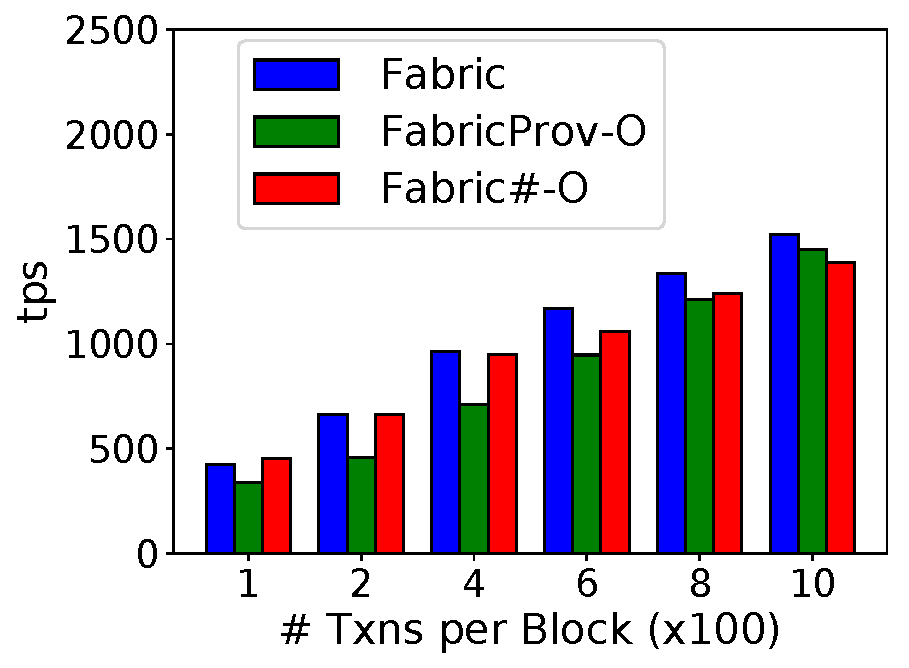
\includegraphics[width=0.99\textwidth]{chart/provenance/ycsb_thruput.pdf}
      \caption{YCSB}
      \label{chart:provenance:basic:ycsb}
    \end{subfigure}
    \begin{subfigure}{0.45\textwidth}
      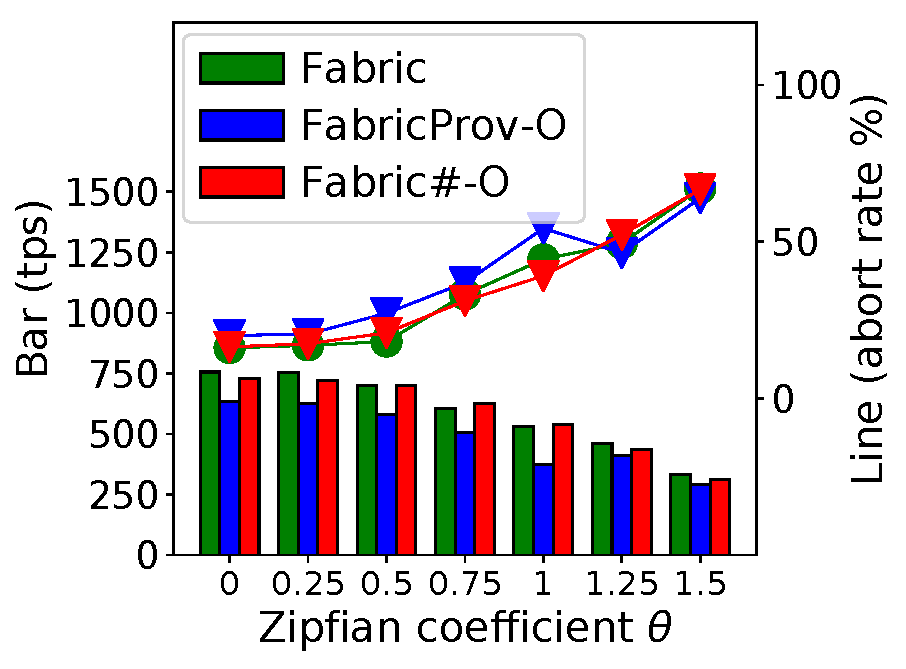
\includegraphics[width=0.99\textwidth]{chart/provenance/smallbank_skew.pdf}
      \caption{Smallbank (skewed)}
      \label{chart:provenance:basic:smallbank_skew}
    \end{subfigure}
    \caption{Effective throughput }
    % \subcaption*{ }
    \label{chart:provenance:basic}
\end{figure}

\subsection{Provenance Overhead and Utility}
\label{sec:provenance:exp:util}
\begin{figure}[tp]
	\centering
    \begin{subfigure}{0.45\textwidth}
      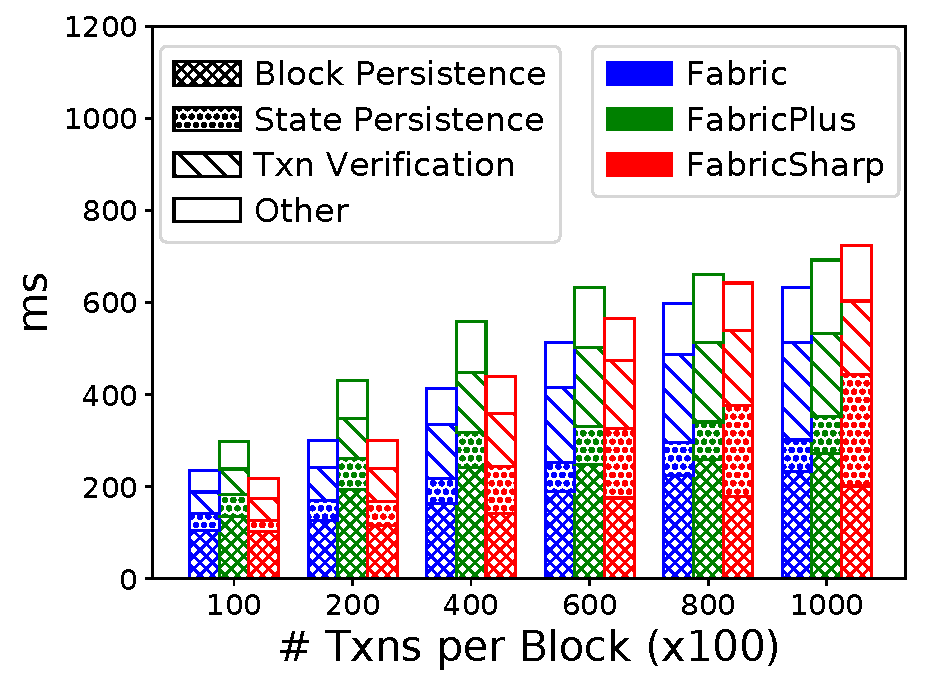
\includegraphics[width=0.99\textwidth]{chart/provenance/ycsb_breakdown.pdf}
      \caption{}
      \label{chart:provenance:ycsb_breakdown}
    \end{subfigure}
    \begin{subfigure}{0.45\textwidth}
      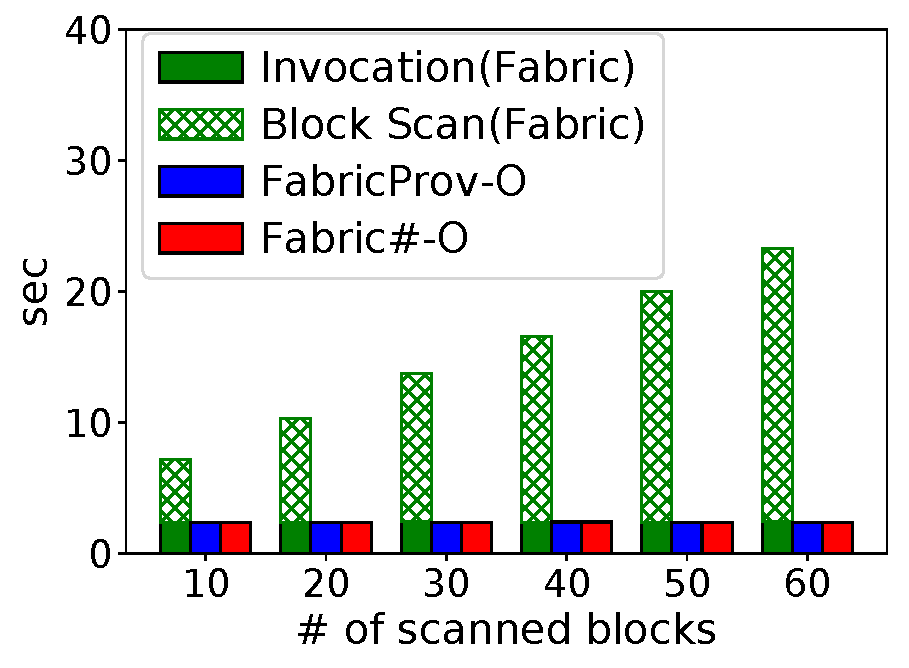
\includegraphics[width=0.99\textwidth]{chart/provenance/smallbank_util.pdf}
      \caption{}
      \label{chart:provenance:smallbank_util}
    \end{subfigure}
    \caption{Provenance overhead and utility }
    \subcaption*{(a) The breakdown of the block validation delay in YCSB (b) The delay to invoke the provenance-dependent \textit{Refund} logic in Smallbank.}
    % \label{chart:provenance:util_overhead}
\end{figure}
Figure~\ref{chart:provenance:ycsb_breakdown} breaks down the latency of block validation into multiple phases, block persistence, state persistence, transaction verification and others. 
As we have demonstrated in Chapter~\ref{sec:twin:exp:replication:model}, the sequential validation rate decides on the system capacity. 
Figure~\ref{chart:provenance:ycsb_breakdown} reveals a greater delay in {\fsPrO}, especially under small blocks. 
In particular, we observe that {\fsPrO} takes $25$\% more time to persist blocks than Fabric and {\fsO}.
By our careful inspection of the codebase, we realize that all Fabric variants construct an index on transactions when persisting a block. 
The index is persisted into the same storage (LevelDB) engine, which also maintains the latest state in Fabric.
However, that storage in {\fsPrO} incurs a heavier role: as explained in Chapter~\ref{sec:provenance:exp:setup}, it tracks all data provenance. 
The overloaded usage accounts for the increased delay to build the transaction index, which ultimately translates into the lower throughput in {\fsPrO}. 
On the other hand,  {\fsO} delegates the provenance tracking responsibility separately to ForkBase. 
It is why the block persistence in {\fsO} saves around $10$\% time compared with Fabric. 
However, {\fsO} takes more than 3 times to persist states (provenance) to ForkBase as Fabric and {\fsPrO} persist states (provenance) to LevelDB. 
For example with 1000 transactions per block, this delay in {\fsO} reports $242$ms while 69ms and 81ms in Fabric and {\fsPrO}.
This is understandable as {\fsO} additionally maintains the DASL and hash DAG for the provenance integrity. 
But fortunately, the delay ratio of the state persistence with respect to the overall block validation is small:
given the overall block validation delay is $723$ms in {\fsO}, this ratio is below $1/3$.
It explains why the total block validation delay in {\fsO} is within $14$\% and $4$\% more than Fabric and {\fsO}. 
So that {\fsO} reports the negligible performance overhead, even though it additionally preserves the provenance with the integrity guarantee.

The provenance-provided utility is abundant. In the Smallbank contract, we additionally encode a provenance-dependent method \texttt{ConditionalRefund}, as attached in Appendix~\ref{sec:append:contracts:cond_refund}.
Similar to the \texttt{Refund} example in Figure~\ref{code:prov:enhanced_contract},
it refunds a bank account with an amount conditional on its involved transactions in recent blocks.
We compare the end-to-end latency of the exact procedure in Fabric, without the provenance support.
Fabric has to break the flow into two phases: first scan blocks for relevant transactions and then invoke the \texttt{Refund} with the self-computed amount.
Figure~\ref{chart:provenance:smallbank_util} demonstrates tremendous utility to expose smart contracts with provenance.
Both {\fsO} and {\fsPrO} are capable to consolidate the above provenance-dependent logic into a single invocation, which takes around 2s. 
In contrast in Fabric, the delay of the sequential block scanning increases with the number of requested recent blocks. 
Even though the block fetching can be done in parallel, 
the separation of two phases is not only error-prone but also security-flawed, as explained in Chapter~\ref{sec:provenance:intro}.

\subsection{Provenance Historical Query}
In the following experiments, we strip away the storage components from {\fsO} and {\fsPrO} for the specific analysis with the tailored workload. 

We first create 500 key-value tuples and then continuously issue update transactions until there are more 10k blocks in the ledger. We use 500 tuples, which is the same number of transactions in a block, so that every block contains a version of every tuple.  
We then execute a query for
the values of a key at different block numbers. Figure~\ref{chart:provenance:ycsb_dist_query} illustrates the query latency with  
increasing block distance from the last block. One can observe that when the distance is small, {\fsO} without DASL has the lowest latency. Without special index support for the query, it performs linear scan from the latest
version. Therefore, it is fast when the requested version is very recent because the number of read is small.
However, its performance degrades quickly as the distance increases. In particular, when the block distance
reaches $128$, the query is $4\times$ slower than {\fsO} with DASL. We observe that the query latency in
{\fsPrO} is independent of the block distance. It is because the query uses storage index directly. {\fsO}
outperforms the other two. Due to DASL, the query latency in {\fsO} is low when the block distance is
large. When the block distance increases, the latency in {\fsO} increases logarithmically, as opposed to
linearly without DASL.  

\begin{figure}[t]
	\centering
    \begin{subfigure}{0.3\textwidth}
      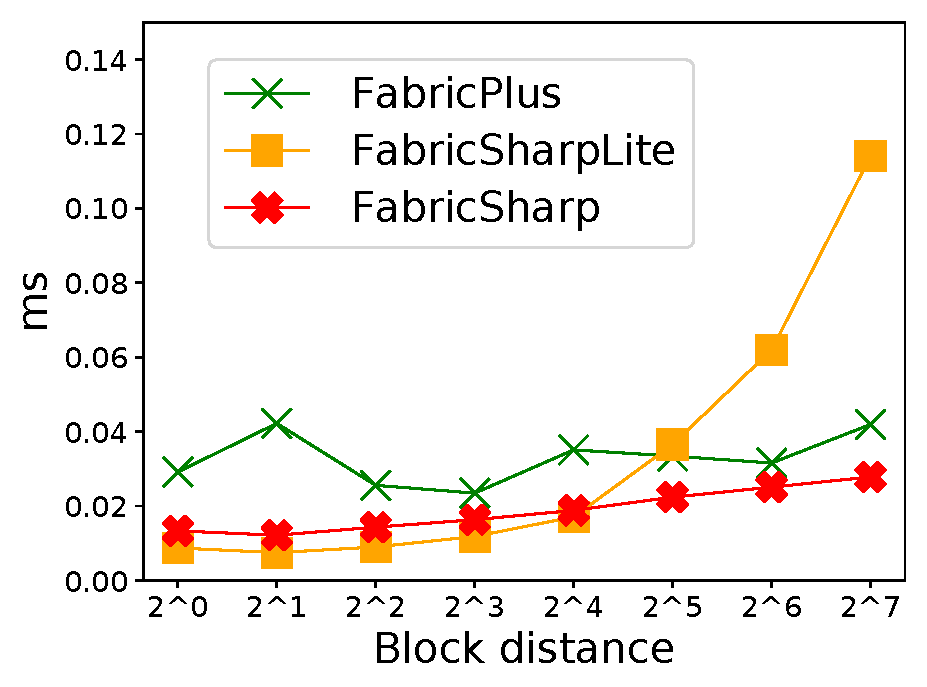
\includegraphics[width=0.99\textwidth]{chart/provenance/ycsb_dist_query.pdf}
      \caption{Version query I}
      \label{chart:provenance:ycsb_dist_query}
    \end{subfigure}
    \begin{subfigure}{0.3\textwidth}
      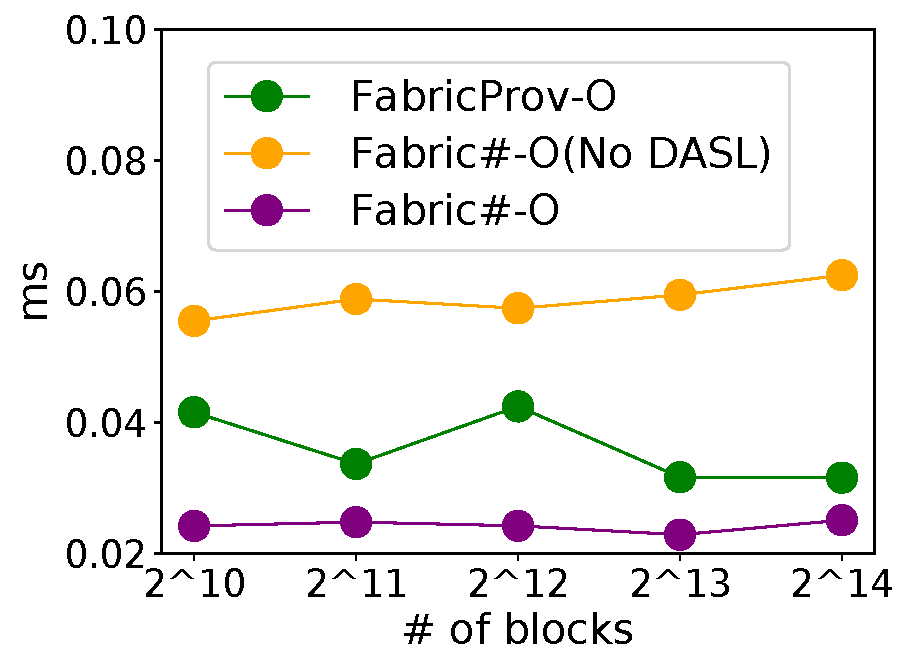
\includegraphics[width=0.99\textwidth]{chart/provenance/ycsb_blk_query.pdf}
      \caption{Version query II}
      \label{chart:provenance:ycsb_blk_query}
    \end{subfigure}
    \begin{subfigure}{0.3\textwidth}
      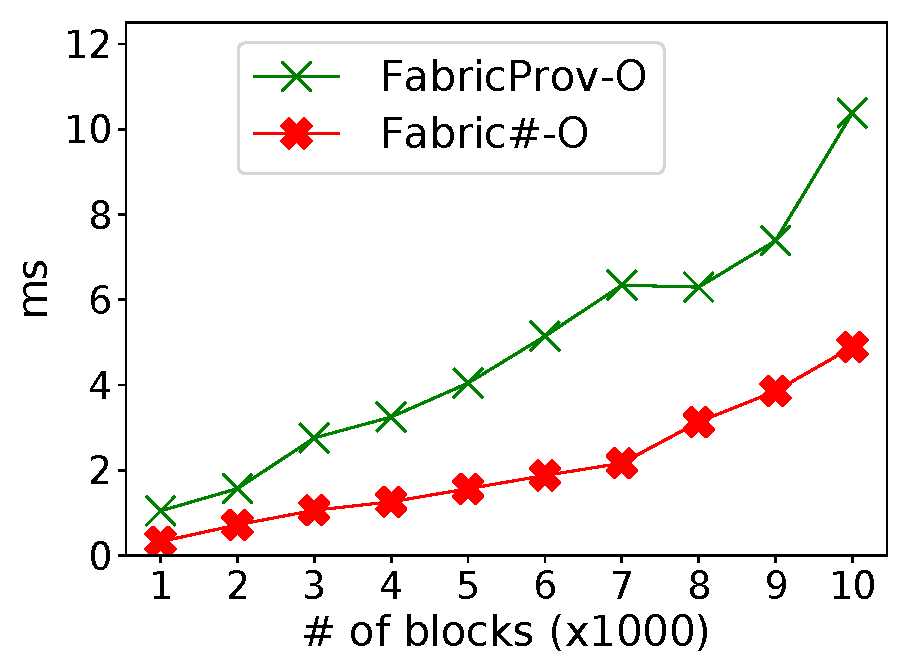
\includegraphics[width=0.99\textwidth]{chart/provenance/ycsb_version_scan.pdf}
      \caption{Version scan}
      \label{chart:provenance:ycsb_version_scan}
    \end{subfigure}
    \caption{Latency of historical queries}
    % \label{chart:provenance:util_overhead}
\end{figure}
We repeat the experiment above while fixing the block distance to $64$ and varying the total number of blocks.
Figure~\ref{chart:provenance:ycsb_blk_query} shows the results for the version query when the number of block increases.
It can be seen that the query latency in both {\fsO} with and without DASL remains roughly the same. In other words,
the performance of version queries in these systems are independent of the block numbers, which is due to the
DAG data model that tracks state versions. But the index reduces the
number of hops needed to be read. An interesting observation is that the latency of {\fsPrO} fluctuates
significantly. We attribute this fluctuation to the log-structure-merge tree index in the storage, in which the
requested version may reside at different levels of the tree when the total number of block increases. 

Next, we measure the latency for the operation that scan the entire version history of a given key.
Figure~\ref{chart:provenance:ycsb_version_scan} shows the scan latency with increasing number of blocks between {\fsPrO} and {\fsO}.  
For {\fsPrO}, we first construct the key range and rely on iterator for the scanning.  As the number of block
increases, the version history becomes longer which accounts for the linear increase in latency in both
systems.  However, {\fsO} outperforms {\fsPrO} by a constant factor. We attribute this difference to ForkBase's
optimizations for version tracking. 


\subsection{Provenance Dependency Query}
\begin{figure}[t]
	\centering
    \begin{subfigure}{0.68\textwidth}
      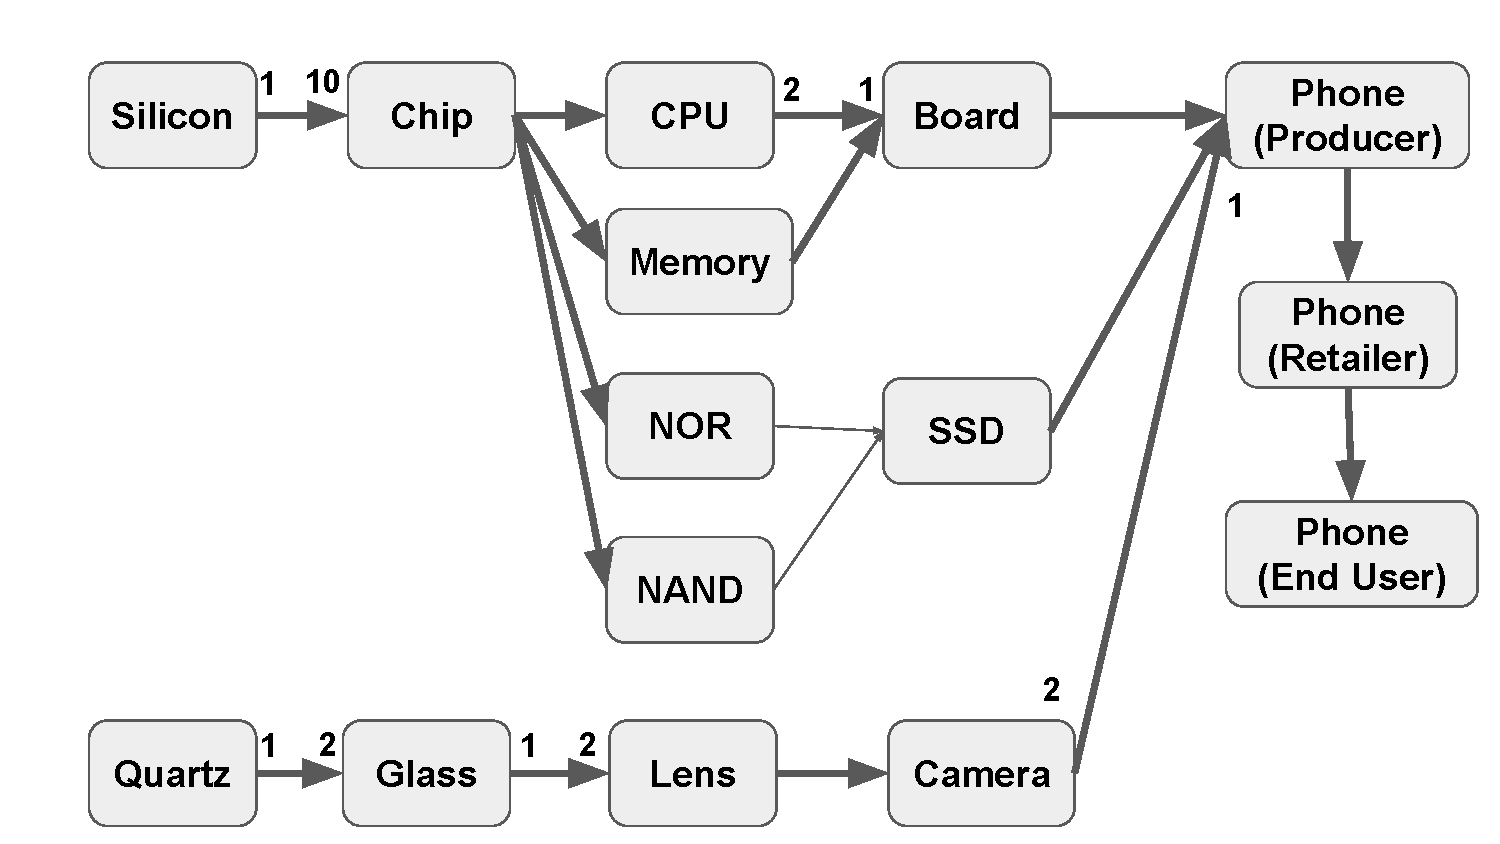
\includegraphics[width=0.99\textwidth]{diagram/provenance/supplychain.pdf}
      \caption{Dependency in the supply chain}
      \label{diagram:provenance:supply_chain_dag}
    \end{subfigure}
    \begin{subfigure}{0.45\textwidth}
      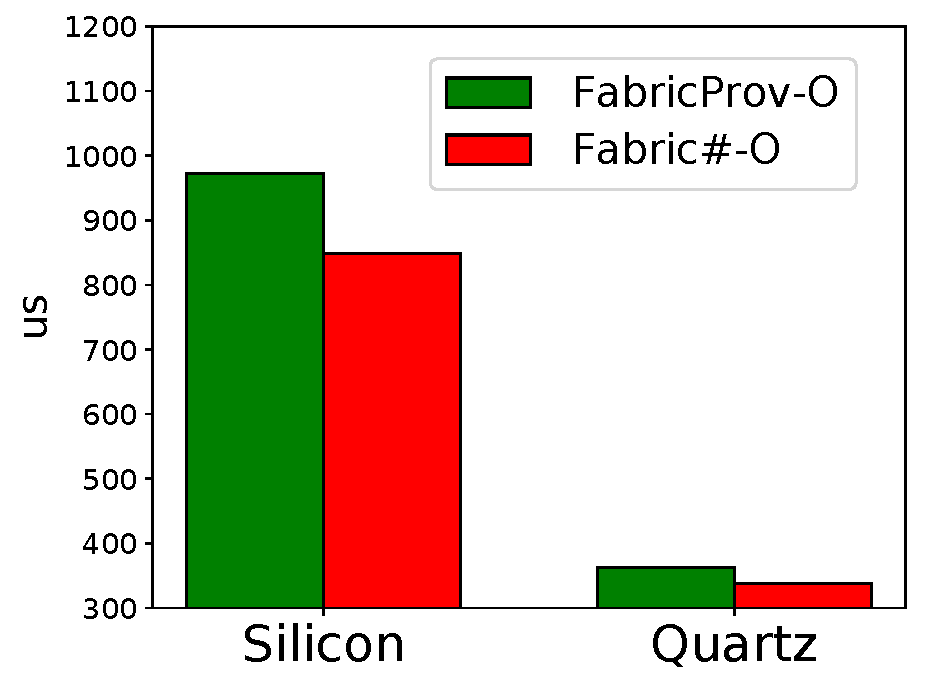
\includegraphics[width=0.99\textwidth]{chart/provenance/forward.pdf}
      \caption{Delay of forward query}
      \label{chart:provenance:supply_chain_forward}
    \end{subfigure}
    \begin{subfigure}{0.45\textwidth}
      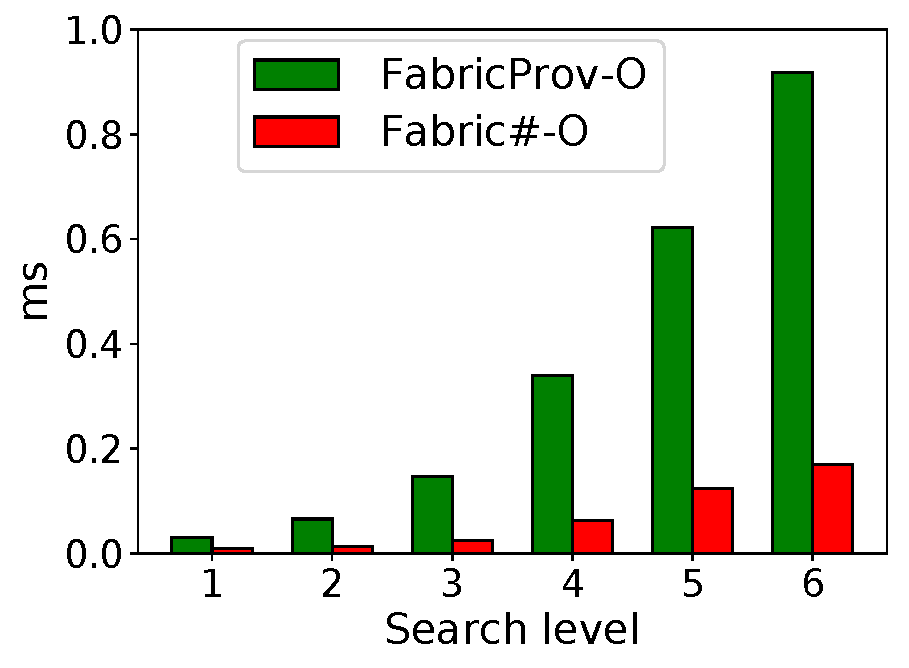
\includegraphics[width=0.99\textwidth]{chart/provenance/bfs.pdf}
      \caption{Delay of BFS traversal}
      \label{chart:provenance:supply_chain_bfs}
    \end{subfigure}
    \caption{Dependency queries on a simulated supply chain}
\end{figure}

For multi-state dependency tracking, we implement a contract for a supply chain
application shown in Figure~\ref{diagram:provenance:supply_chain_dag}.  In this application, a phone is assembled from intermediary
components which are made from other components or raw material. 
We pre-populate raw materials in both {\fsPrO} and {\fsO} and then issue transactions for the above transformation process. 
Each transaction consumes (reads) the source materials and generates (writes) new components. 
The steps after the phone production represent ownership changes from producers, retailers and end users.
This supply chain is more complex than the example in Figure~\ref{code:prov:contract}, as it consists of a DAG with
maximum depth of $6$. We generate synthetic data for this contract, and measure the latency of operations
using  \texttt{Forward} and \texttt{Backward} version tracking.

We evaluate the query performance with multi-state dependency. We populate the blockchain states with
raw materials and issue transactions that create new phones.  We perform two experiments. First, we assume
that one piece of silicon and quartz is found defected, and use forward tracking to find the
affected materials and phones. Second, we perform a standard DAG traversals, breadth-first search (BFS), to retrieve all the dependencies of a phone. 
Figure~\ref{chart:provenance:supply_chain_forward} compares the latency of forward tracking, and Figure
\ref{chart:provenance:supply_chain_bfs} shows the BFS traversal performance with varying depths.  For forward tracking, we observe that
{\fsO}'s delay is 10\% smaller than that of {\fsPrO}.  It takes less time to track the affected quartz than
the affected the silicon, because the silicon is at a deeper position in the supply
chain.  The gap between {\fsO} and {\fsPrO} is much more evident in the BFS traversal, 
in which the latencies of both systems grow exponentially with increasing depths.  However,
{\fsO} outperforms the baseline.  It is because the index in {\fsO} directly captures the dependencies,
whereas each backtrack operation in {\fsPrO} requires traversing the storage index.  As the number of queries
increases with the search depth, their performance gap accumulates.  

\subsection{Provenance Storage}
\begin{figure}[tp]
	\centering
    \begin{subfigure}{0.45\textwidth}
      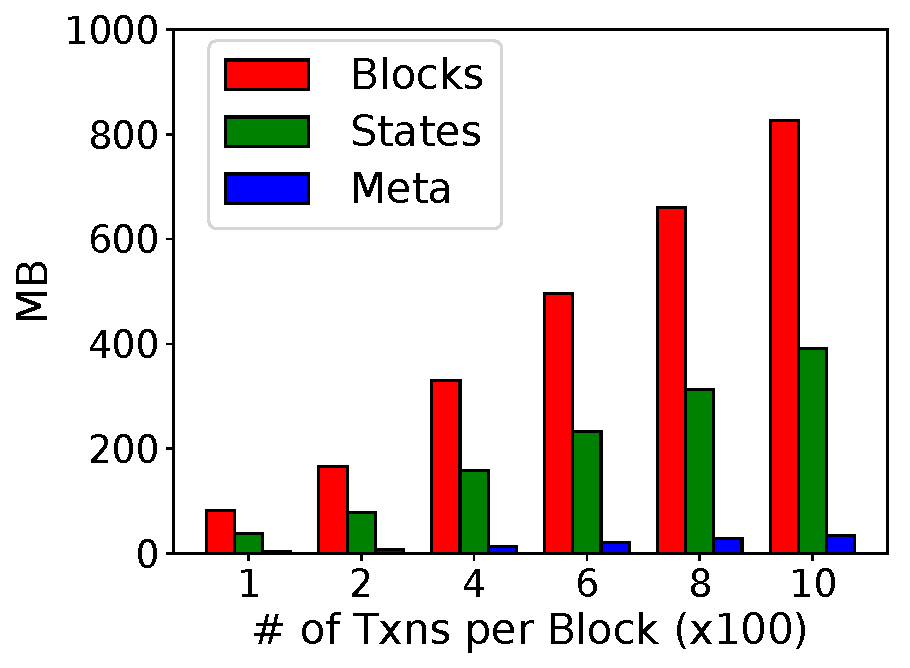
\includegraphics[width=0.99\textwidth]{chart/provenance/ycsb_blksize_storage.pdf}
      \caption{}
      \label{chart:provenance:ycsb_blksize_storage}
    \end{subfigure}
    \begin{subfigure}{0.45\textwidth}
      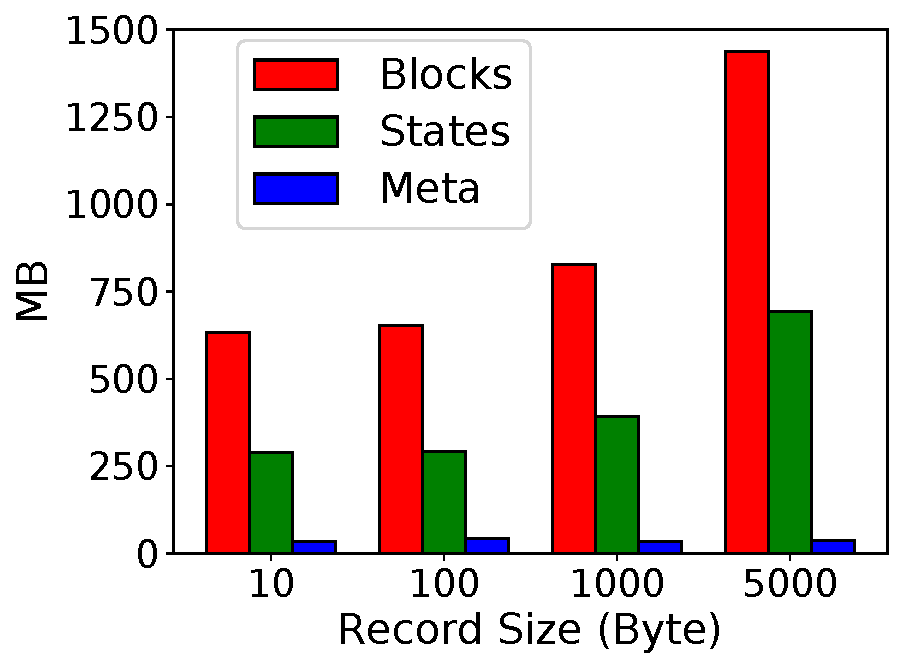
\includegraphics[width=0.99\textwidth]{chart/provenance/ycsb_recordsize_storage.pdf}
      \caption{}
      \label{chart:provenance:ycsb_recordsize_storage}
    \end{subfigure}
    \caption{Provenance storage size}
    \subcaption*{The storage space with (a) the varying block size and fixed record size (1000 bytes) (b) the varying record size and the fixed block size (1000 transactions per block). \textit{Meta} measures the size for all provenance information, such as hash pointers of Merkle DAG and DASL. }
    % \label{chart:provenance:util_overhead}
\end{figure}
In the last experiment, we populate 100 blocks with the YCSB workload. 
We place our focus solely on {\fsO} to understand the storage constitution for a blockchain application. 
Even though there might be differences if with {\fsPrO}, the differences are specific to their storages, that is, ForkBase in {\fsO} and LevelDB in{\fsPrO}. 
Their comparison is out of the scope. 

We measure the consumed storage space with the varying block size and the record size, 
which are respectively reported in Figure~\ref{chart:provenance:ycsb_blksize_storage} and~\ref{chart:provenance:ycsb_recordsize_storage}. 
One can observe that the storage consumption grows linearly with the number of blocks. 
The storage increase is not evident until the record size grows to 5000 bytes. 
But the block content constantly accounts for the majority of the storage cost.
In particular, despite the different settings, blocks occupy around $66$\% of the entire space. 
The result further confirms the conclusion drawn in Chapter~\ref{sec:twin:exp:storage}: compared with the state storage, the ledger abstraction incurs the most storage overhead. 
But to our astonishment, we find that the storage consumption for data provenance is far less than expected, as shown in the negligible \texttt{Meta} bar. 
Their storage ratios are all below $1$\% when a block contains 1000 transactions. 
In the worst case with 100 transactions per block, the ratio is only $6.7$\%.
Hence we conclude that the storage overhead for the extra provenance and DASL index is insignificant. 
